\graphicspath{{./chapters/ncov-forecasting-fit/}}
\chapter{Supplementary Materials for Chapter 3} 

\section{Supplementary Figures}

% TODO: Return to figure references!

% Include only the SI item label in the paragraph heading. Use the \nameref{label} command to cite SI items in the text.
% \paragraph*{S1 Fig}
%
% \label{fig:S1}
% {\bf Reconstructing available data sets for Australia, Brazil, South Africa, Trinidad and Tobago, the United Kingdom, and Vietnam.}
% (A) Variant sequence counts categorized by Nextstrain clade at 4 different analysis dates.

\begin{figure}[th!]
	\centering
	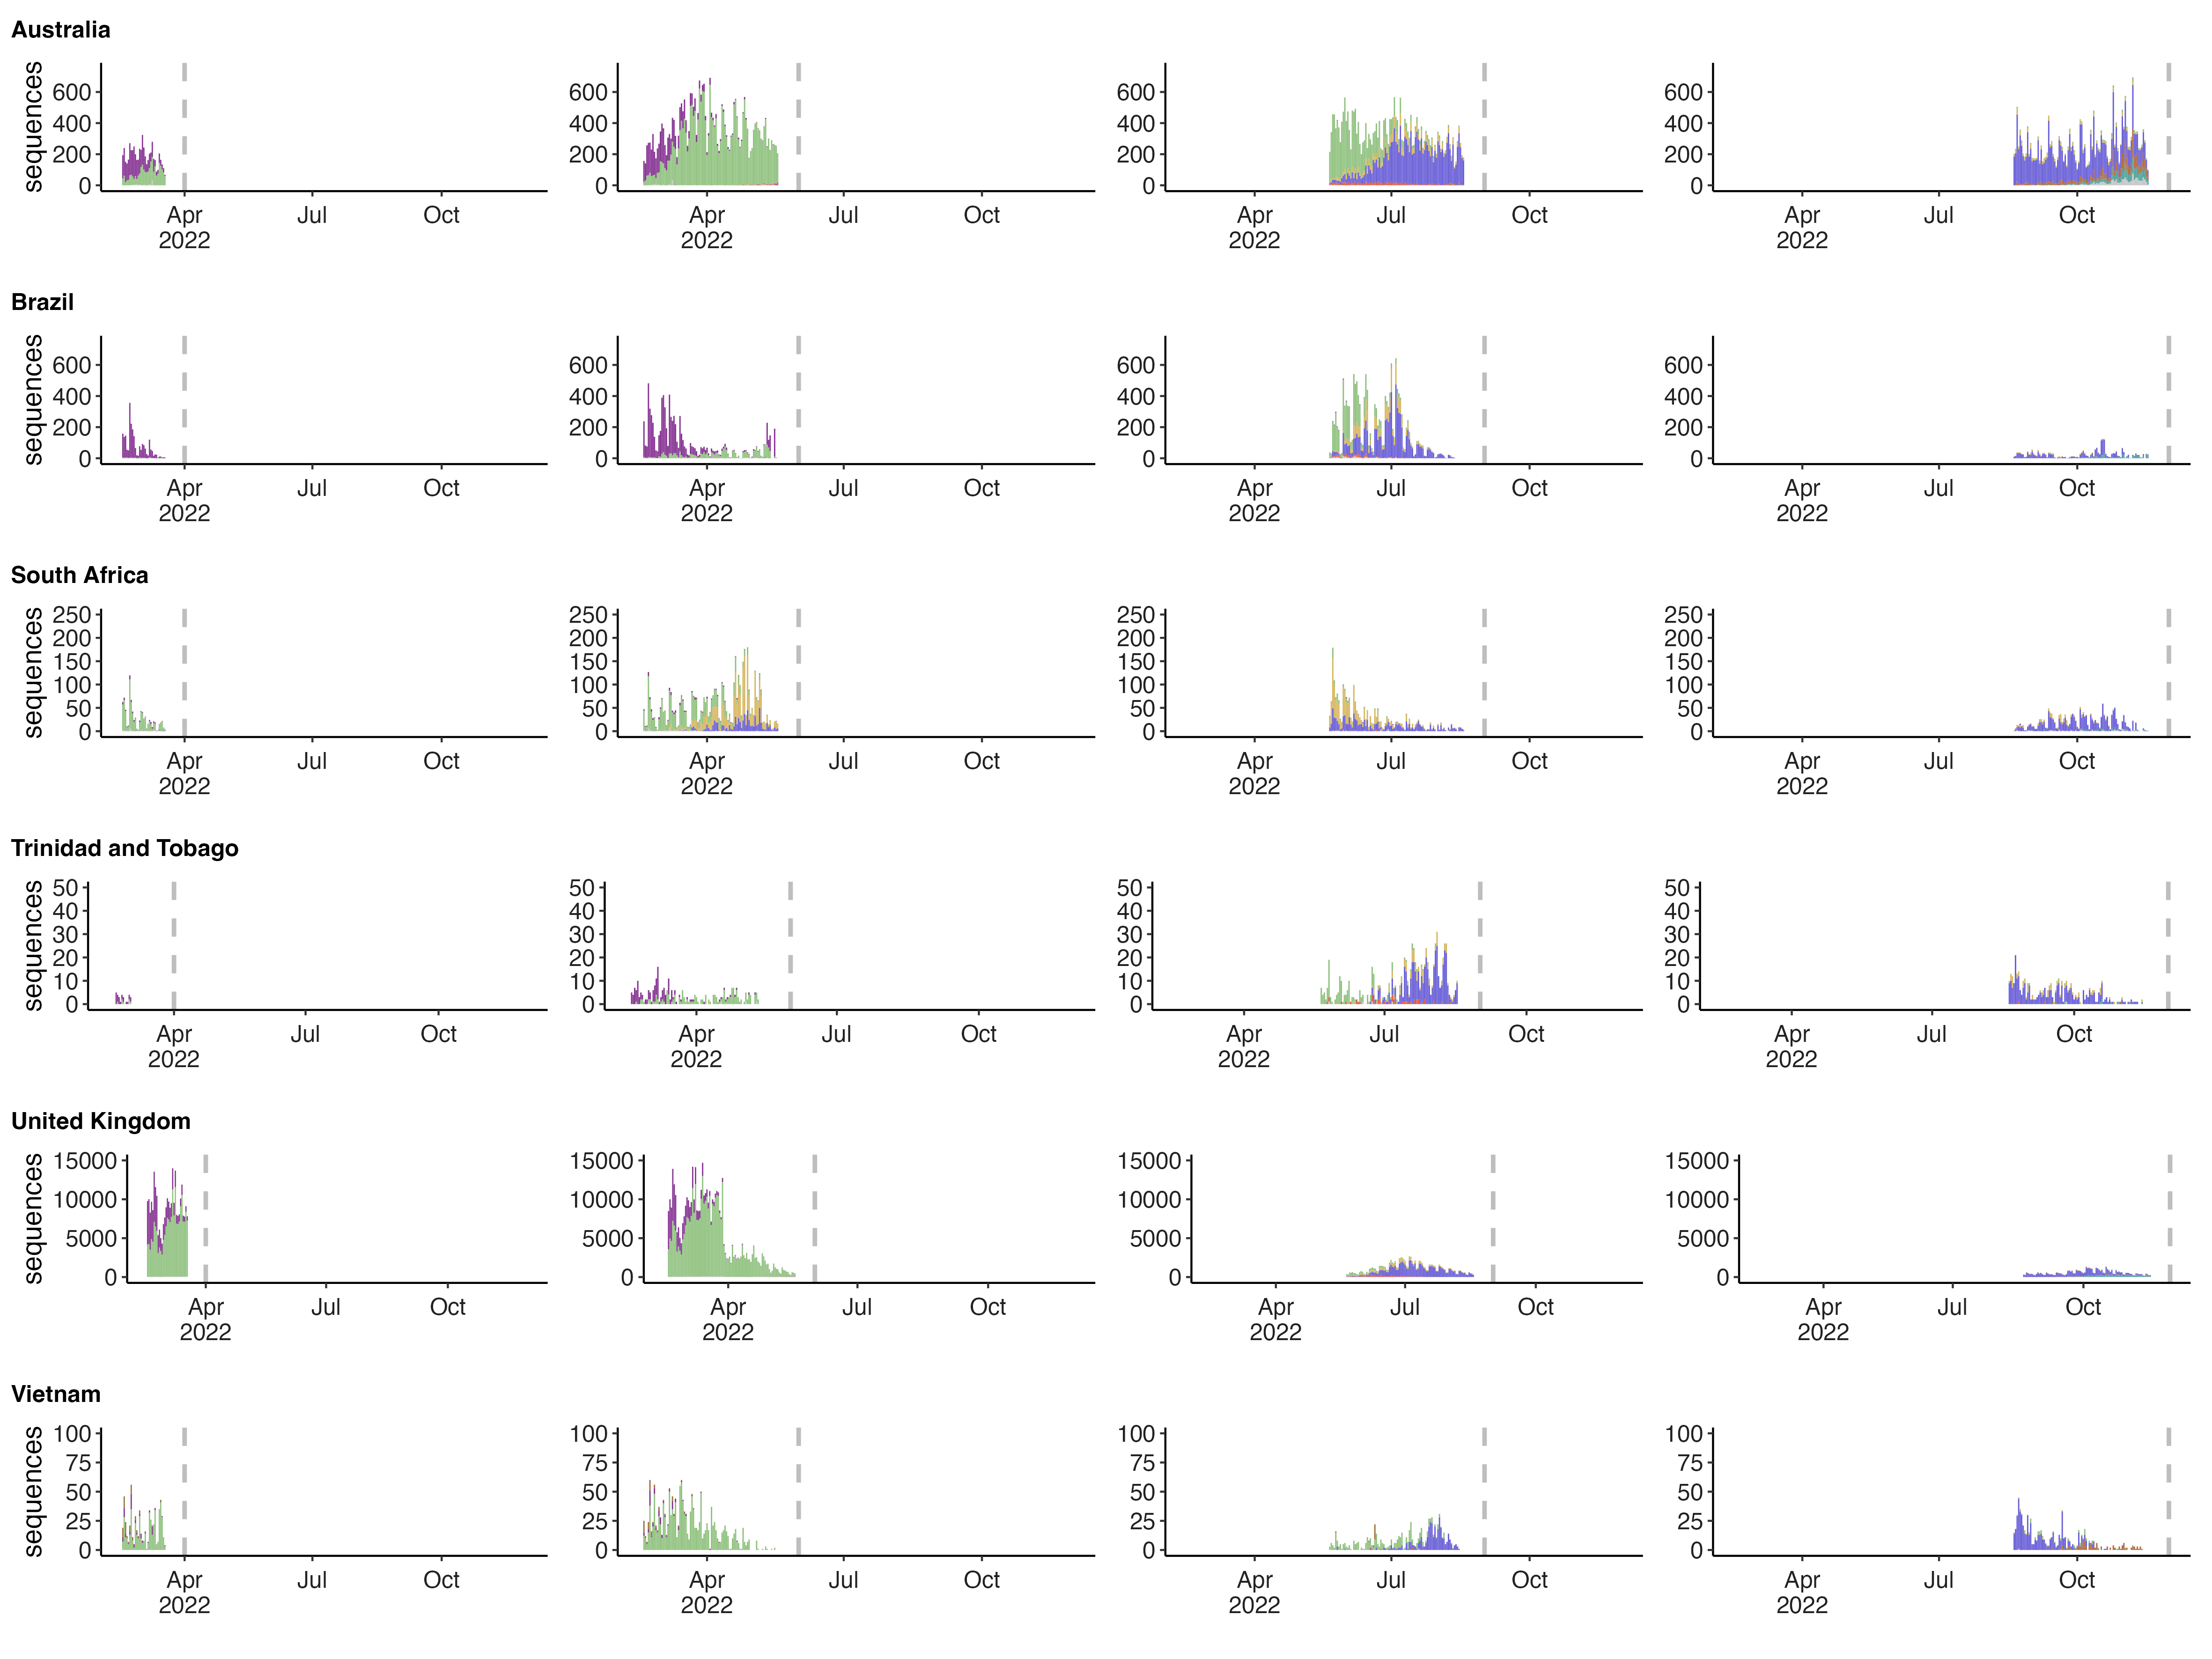
\includegraphics[width=0.9\textwidth=0.01]{supp_figures/Supplementary_Fig_1A.png}
	\caption[\textbf{Reconstructing available data sets for Australia, Brazil, South Africa, Trinidad and Tobago, the United Kingdom, and Vietnam.}]{
		\textbf{Reconstructing available data sets for Australia, Brazil, South Africa, Trinidad and Tobago, the United Kingdom, and Vietnam.}
		(A) Variant sequence counts categorized by Nextstrain clade at 4 different analysis dates.
	}
	\label{fig:S1}
\end{figure}

% \paragraph*{S2 Fig}
% \label{fig:S2}
% {\bf Reconstructing predictions for Australia}
% (A) +30 day frequency forecasts for variants in bimonthly intervals using the MLR model for Australia.
%                 Each forecast trajectory is shown as a different colored line.
%                 Retrospective smoothed frequency is shown as a thick black line.

\begin{figure}[th!]
	\centering
	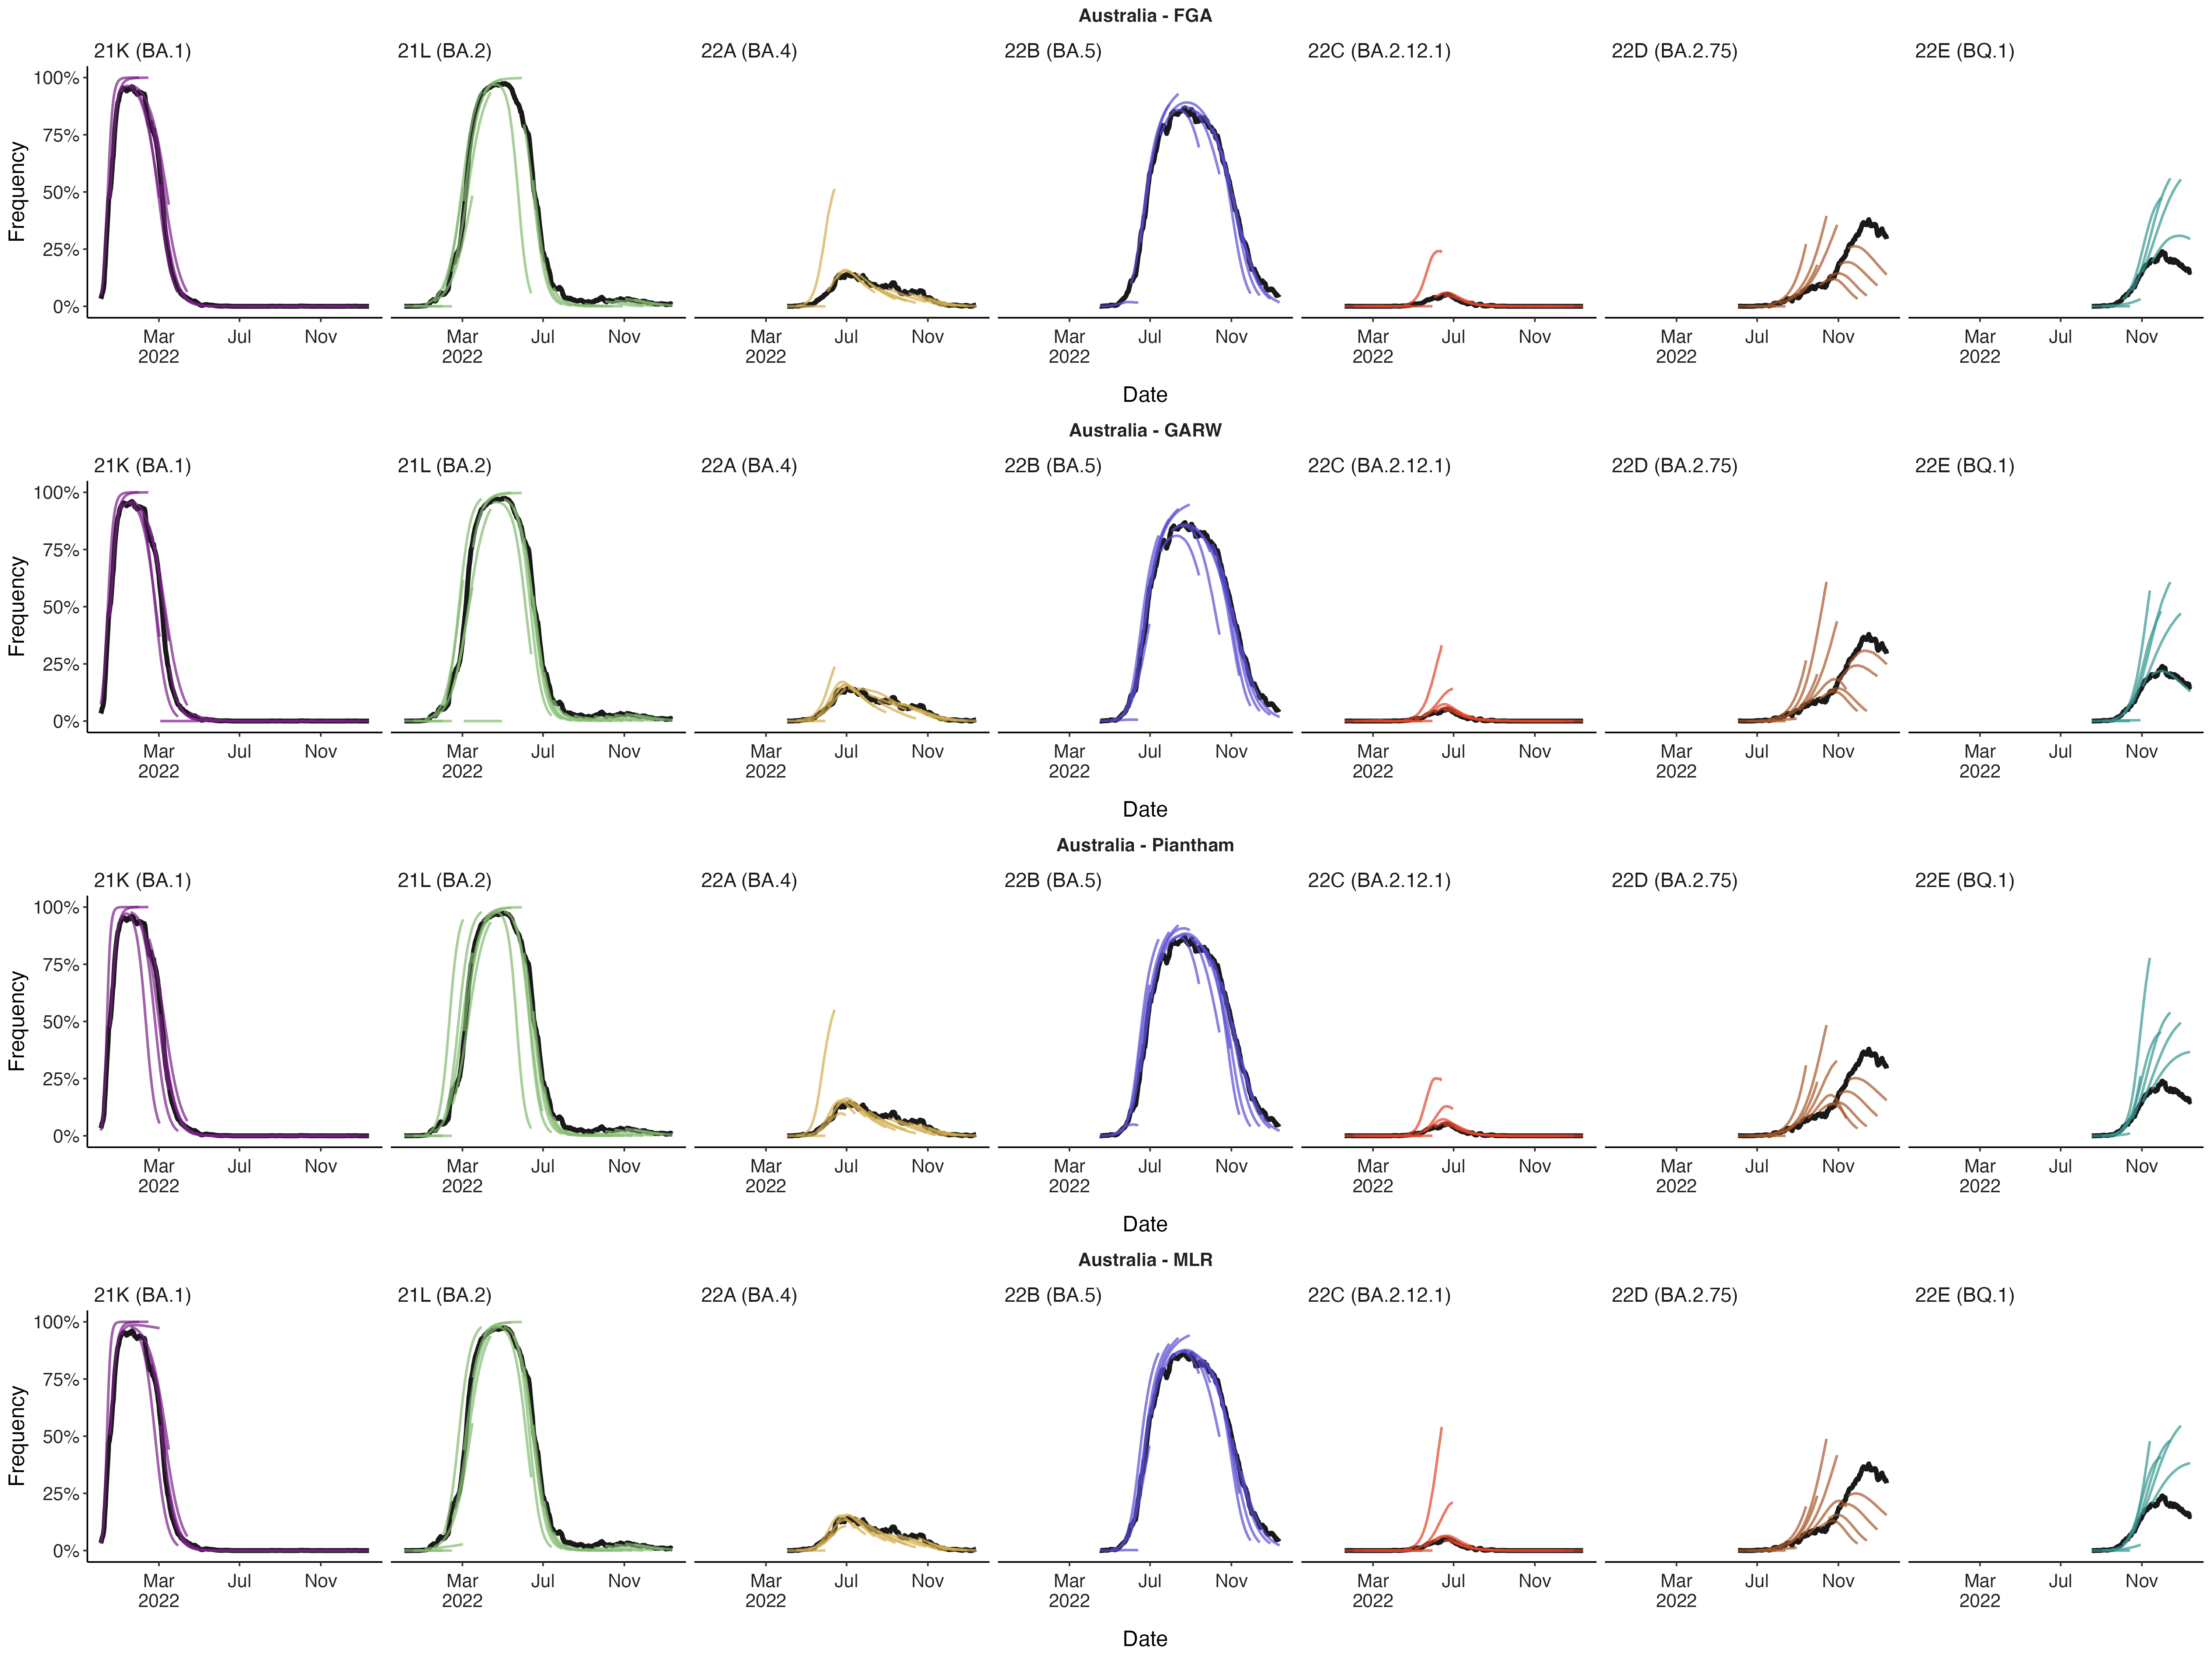
\includegraphics[width=0.9\textwidth=0.01]{supp_figures/supplementary_fig_Australia.png}
	\caption[\textbf{Reconstructing predictions for Australia}]{
		\textbf{Reconstructing predictions for Australia}
		(A) +30 day frequency forecasts for variants in bimonthly intervals using the MLR model for Australia.
		Each forecast trajectory is shown as a different colored line.
		Retrospective smoothed frequency is shown as a thick black line.
	}
	\label{fig:S2}
\end{figure}


% \paragraph*{S3 Fig}
% \label{fig:S3}
% {\bf Reconstructing predictions for Brazil}
% (A) +30 day frequency forecasts for variants in bimonthly intervals using the MLR model for Brazil.
%                 Each forecast trajectory is shown as a different colored line.
%                 Retrospective smoothed frequency is shown as a thick black line.

\begin{figure}[th!]
	\centering
	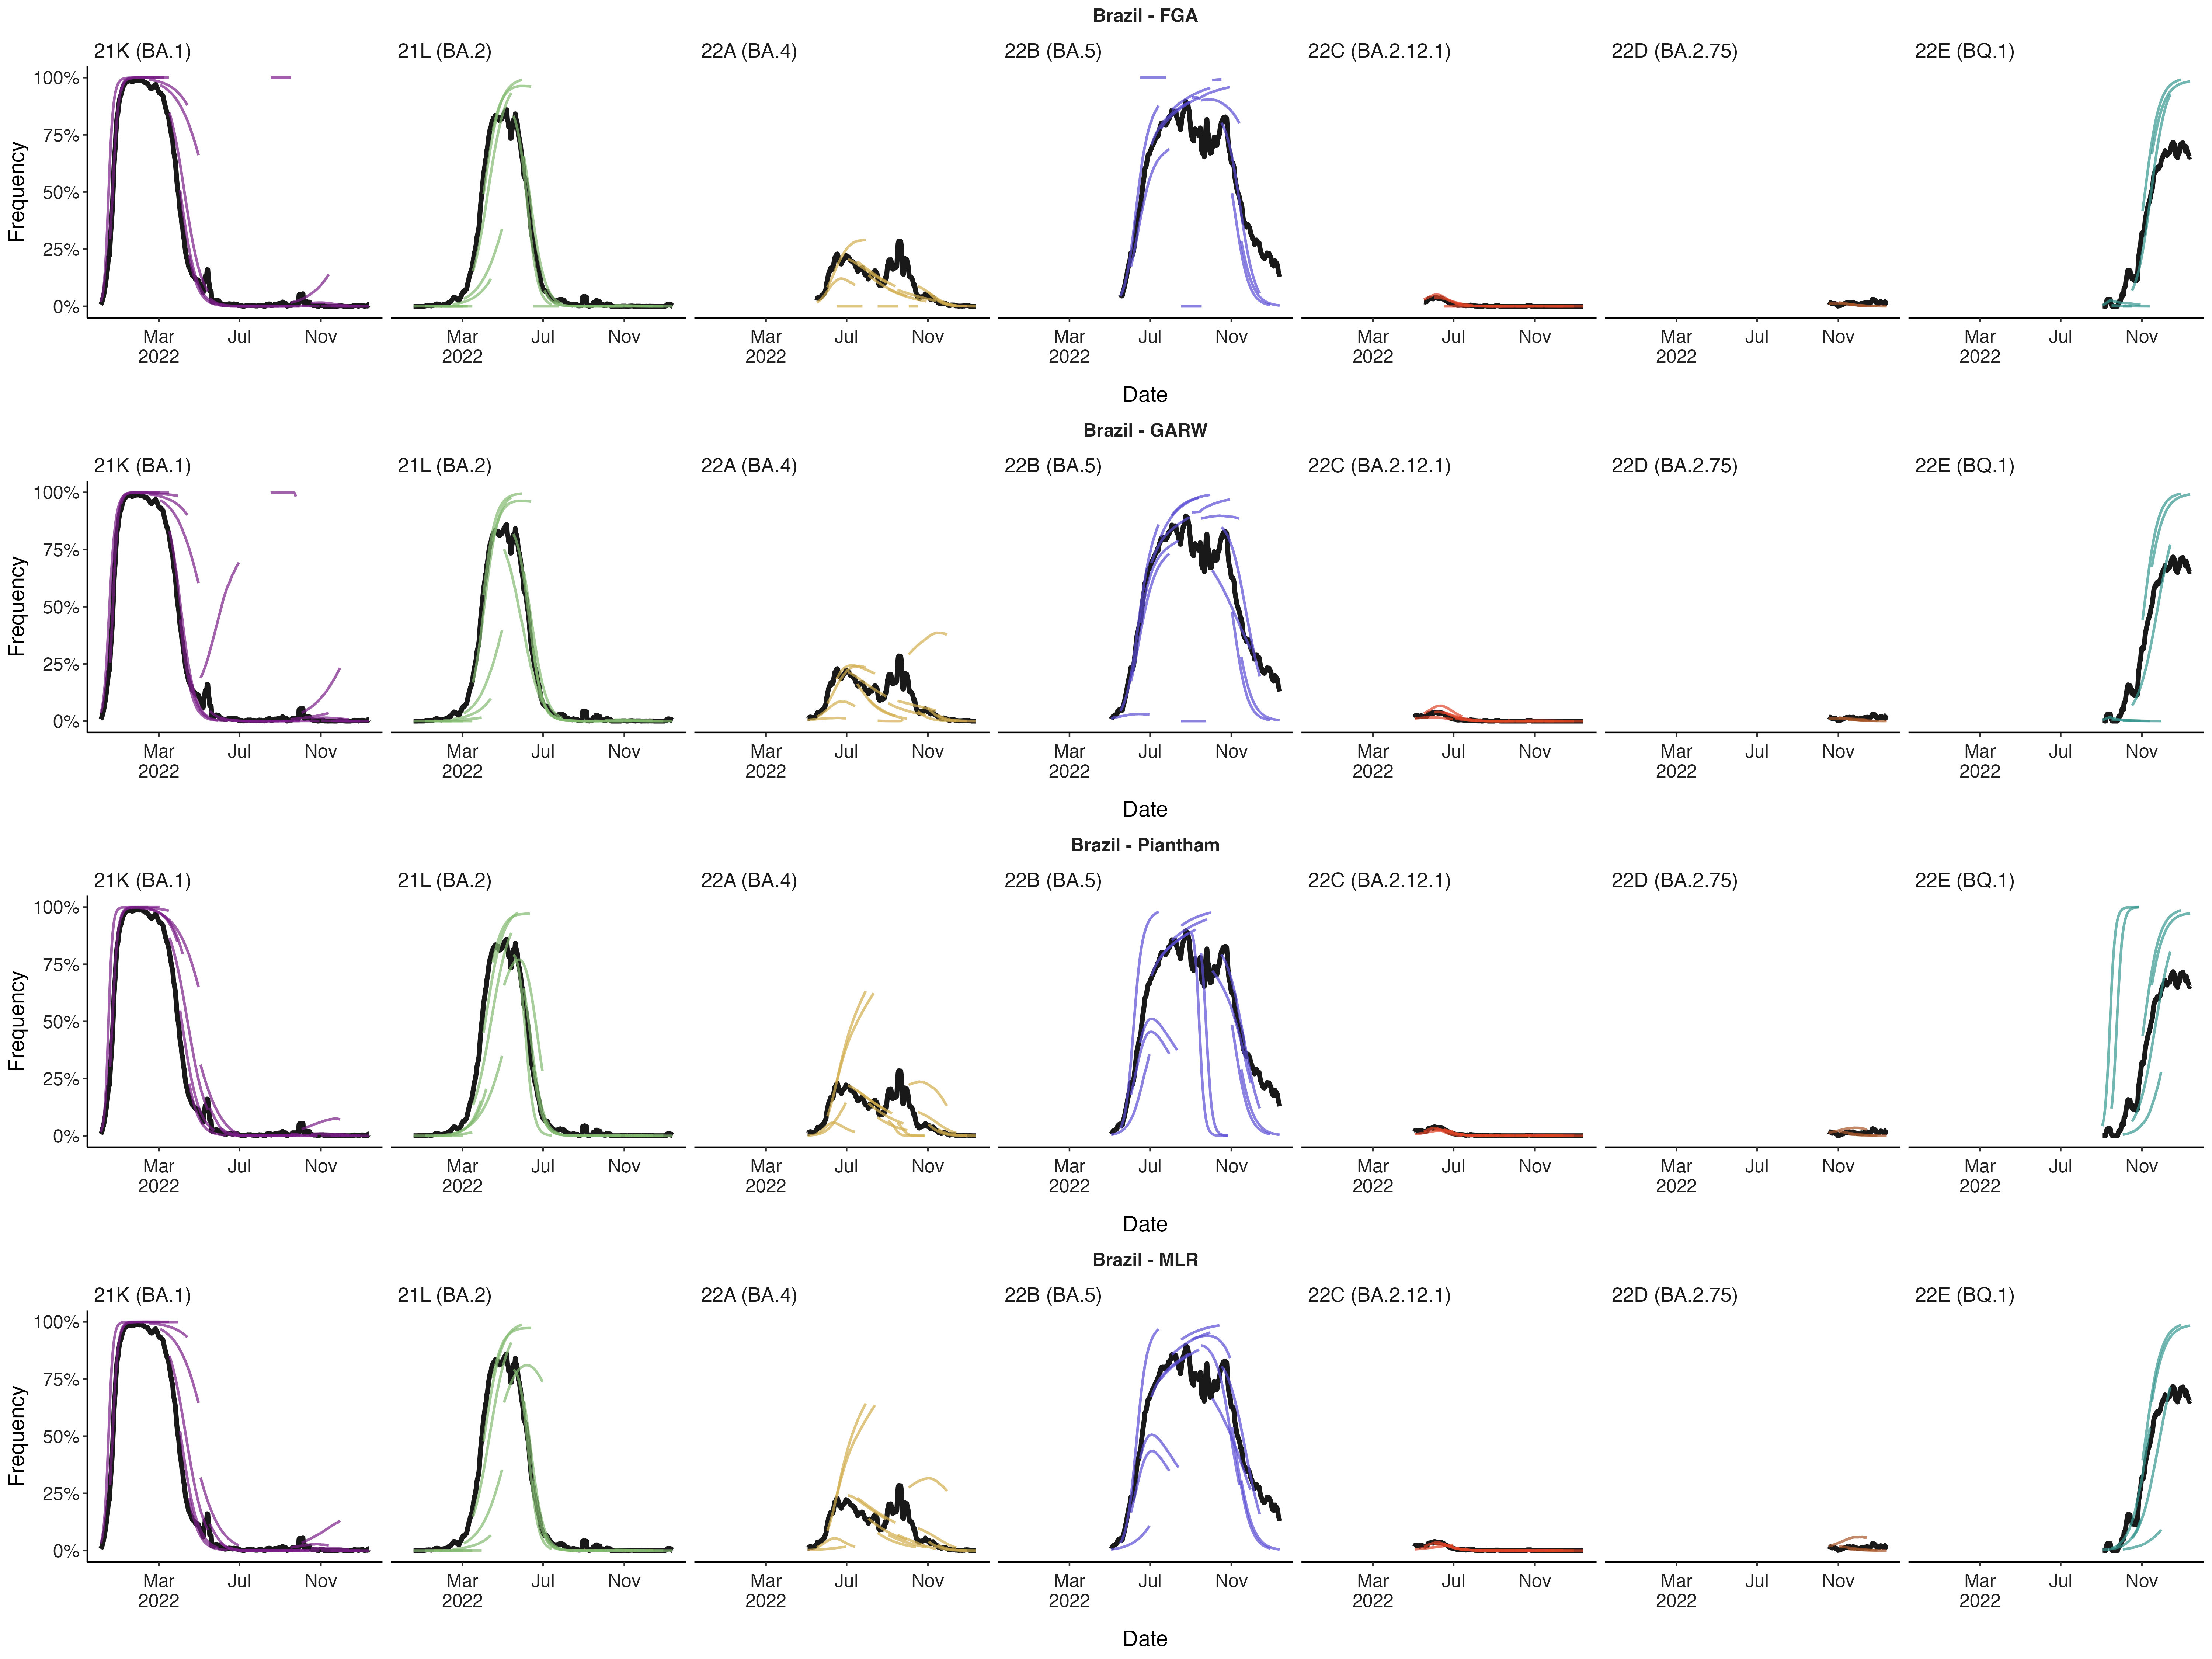
\includegraphics[width=0.9\textwidth=0.01]{supp_figures/supplementary_fig_Brazil.png}
	\caption[\textbf{Reconstructing predictions for Brazil}]{
		\textbf{Reconstructing predictions for Brazil}
		(A) +30 day frequency forecasts for variants in bimonthly intervals using the MLR model for Brazil.
		Each forecast trajectory is shown as a different colored line.
		Retrospective smoothed frequency is shown as a thick black line.
	}
	\label{fig:S3}
\end{figure}

% \paragraph*{S4 Fig}
% \label{fig:S4}
% {\bf Reconstructing predictions for South Africa}
% (A) +30 day frequency forecasts for variants in bimonthly intervals using the MLR model for South Africa.
%                 Each forecast trajectory is shown as a different colored line.
%                 Retrospective smoothed frequency is shown as a thick black line.

\begin{figure}[th!]
	\centering
	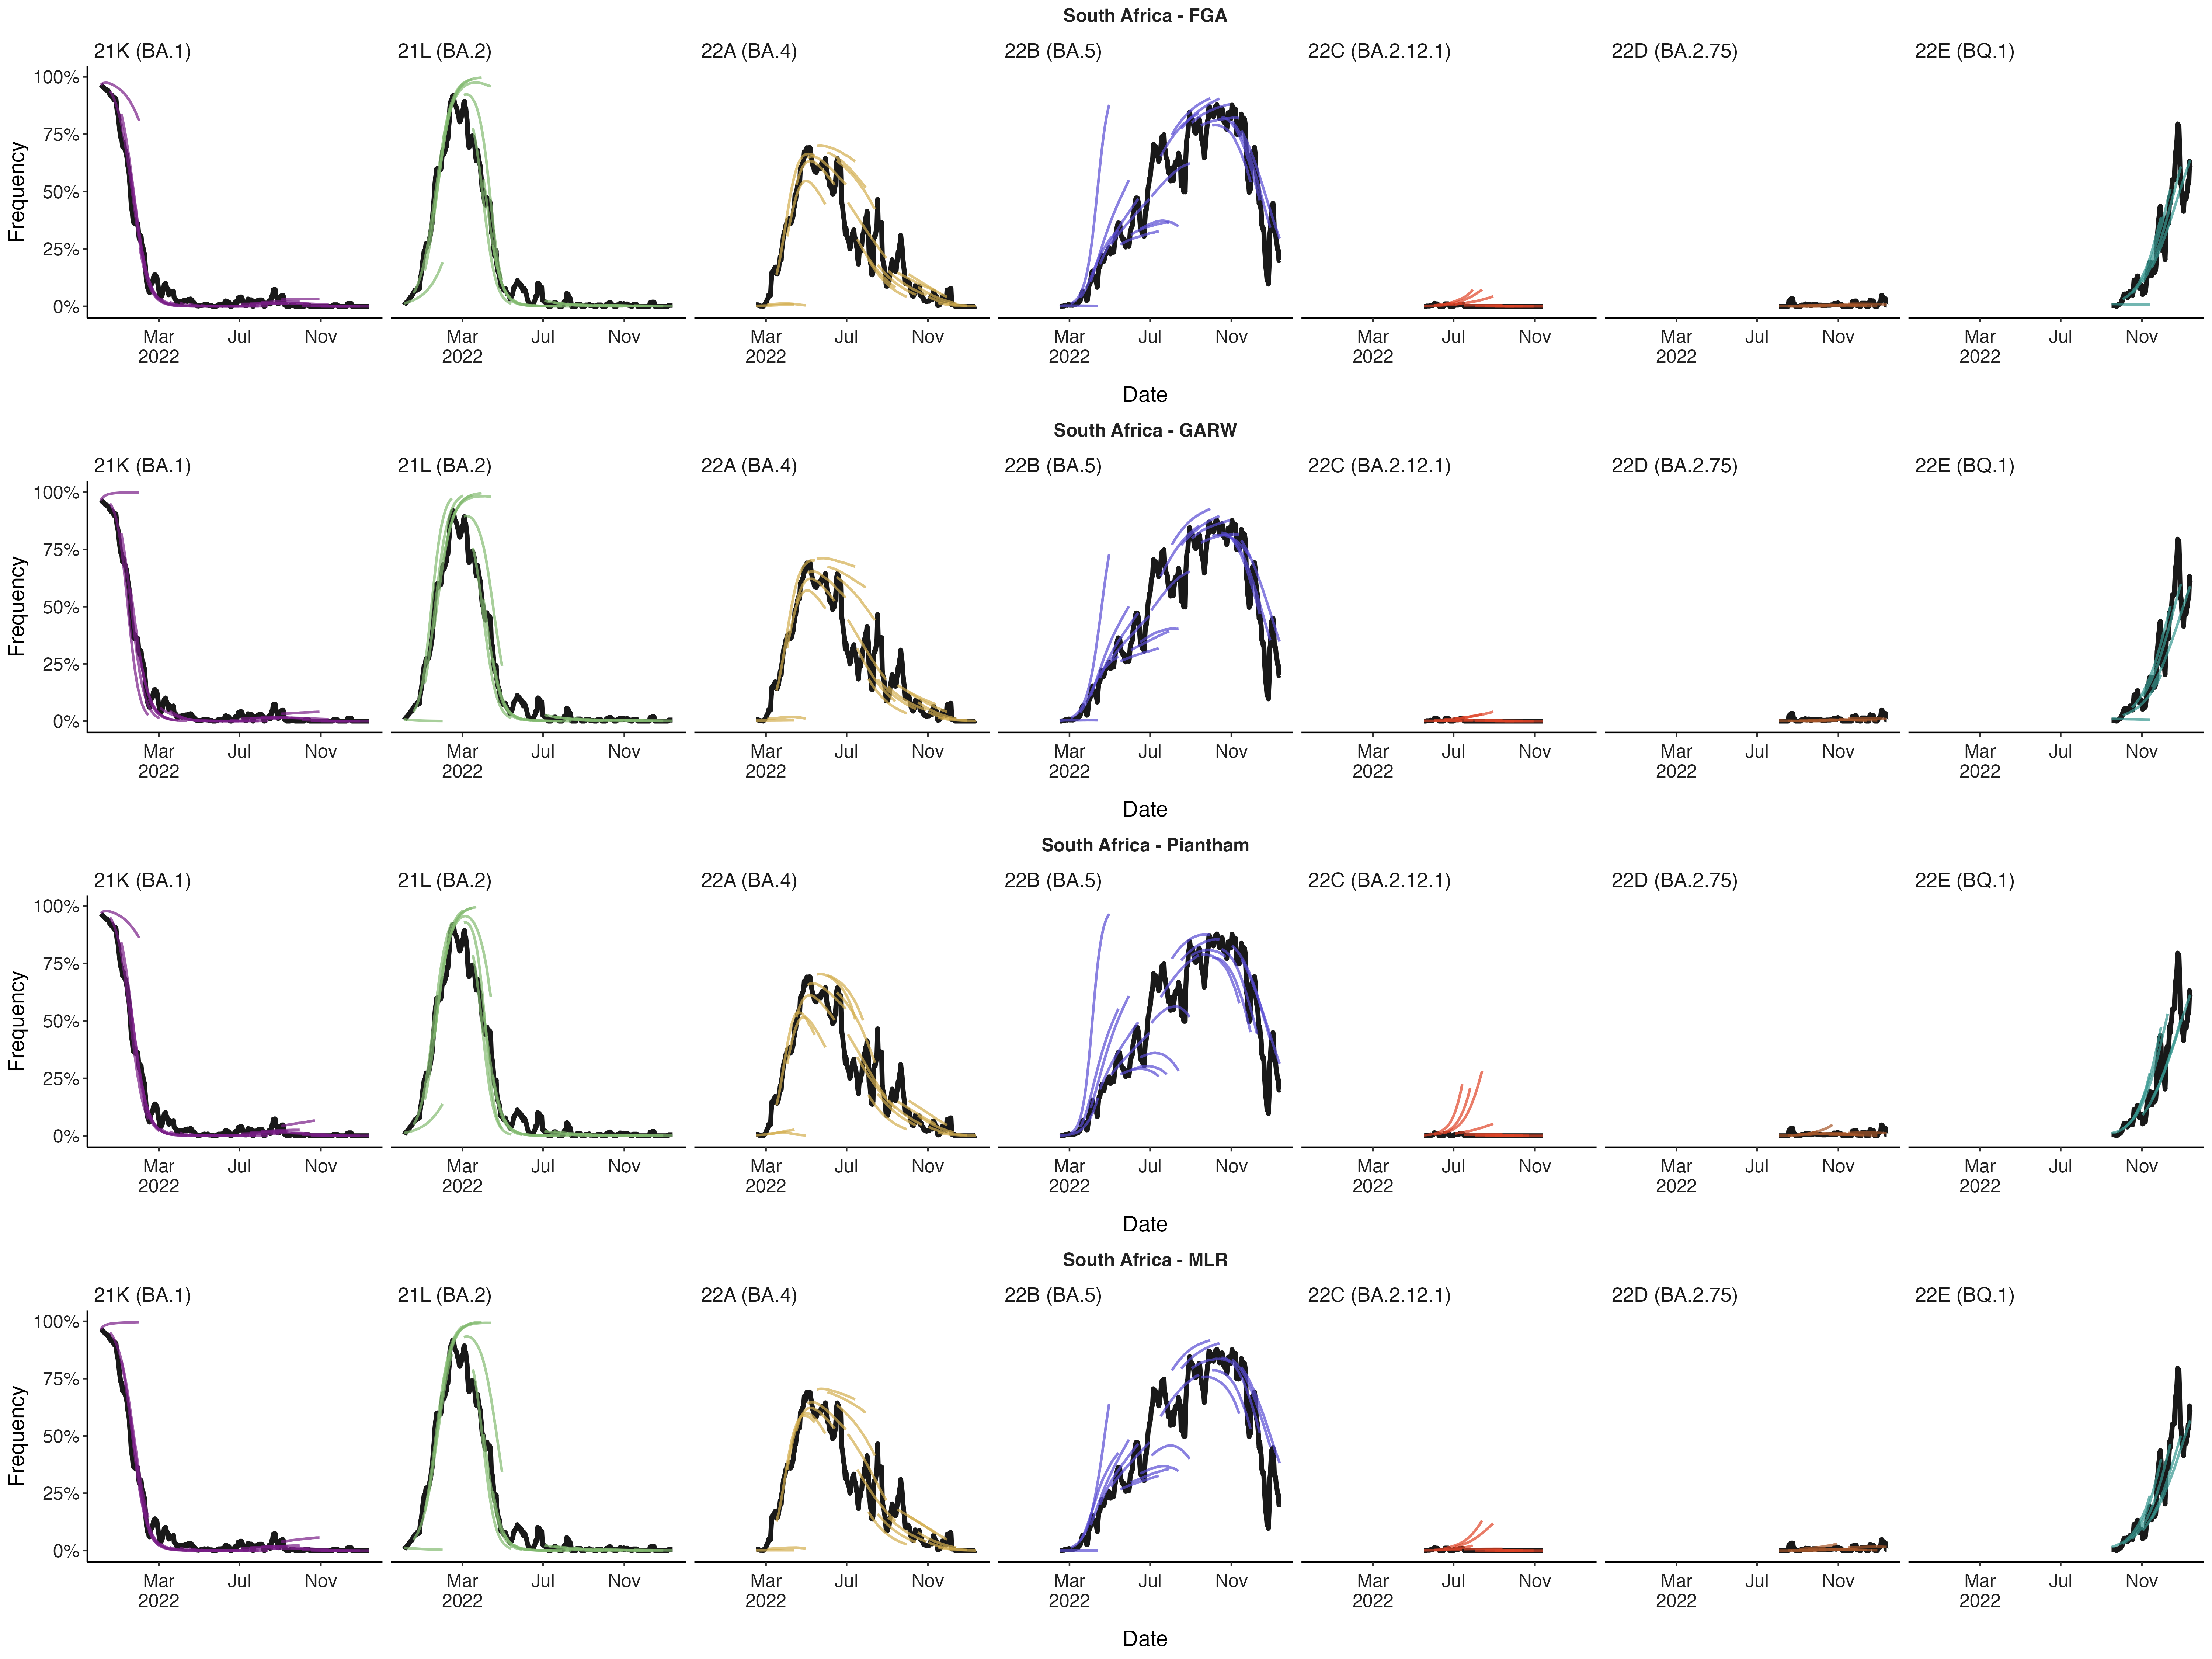
\includegraphics[width=0.9\textwidth=0.01]{supp_figures/supplementary_fig_South Africa.png}
	\caption[\textbf{Reconstructing predictions for South Africa}]{
		\textbf{Reconstructing predictions for South Africa}
		(A) +30 day frequency forecasts for variants in bimonthly intervals using the MLR model for South Africa.
		Each forecast trajectory is shown as a different colored line.
		Retrospective smoothed frequency is shown as a thick black line.
	}
	\label{fig:S4}
\end{figure}

% \paragraph*{S5 Fig}
% \label{fig:S5}
% {\bf Reconstructing predictions for Trinidad and Tobago}
% (A) +30 day frequency
% forecasts for variants in bimonthly intervals using the MLR model for Trinidad and Tobago. Each
% forecast trajectory is shown as a different colored line. Retrospective smoothed frequency is shown
% as a thick black line.

\begin{figure}[th!]
	\centering
	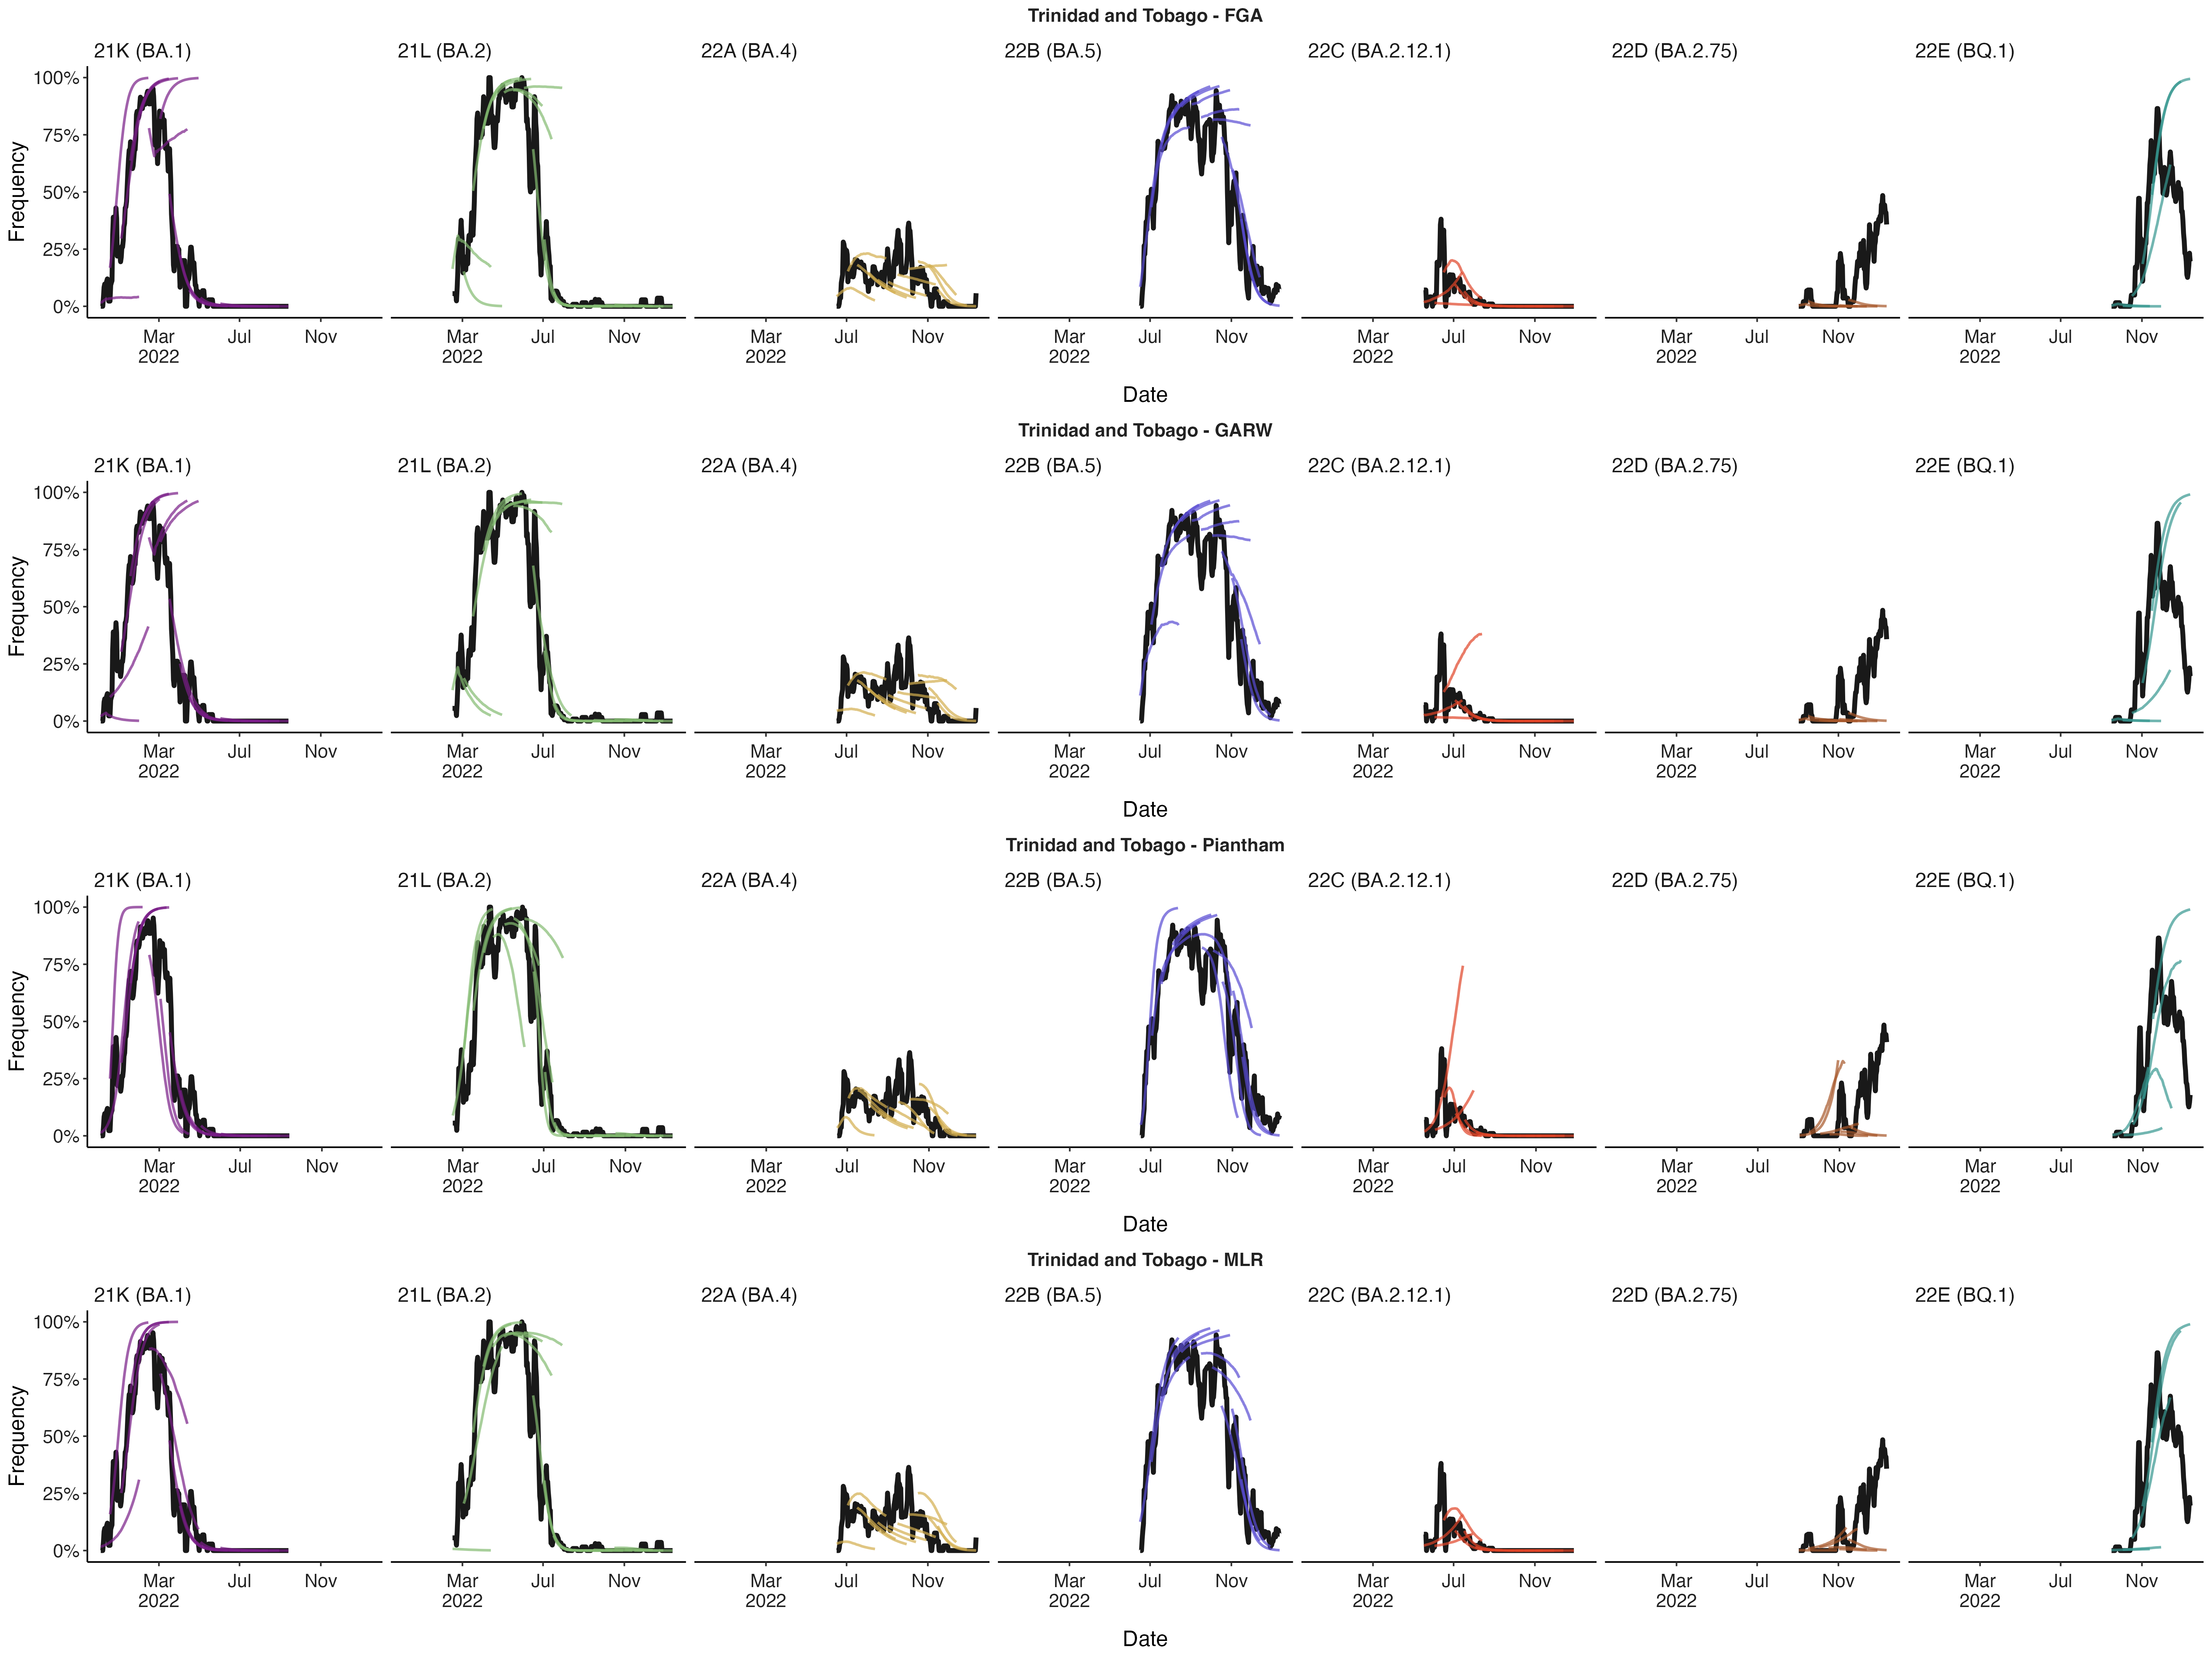
\includegraphics[width=0.9\textwidth=0.01]{supp_figures/supplementary_fig_Trinidad and Tobago.png}
	\caption[\textbf{Reconstructing predictions for Trinidad and Tobago}]{
		\textbf{Reconstructing predictions for Trinidad and Tobago}
		(A) +30 day frequency forecasts for variants in bimonthly intervals using the MLR model for Trinidad and Tobago.
		Each forecast trajectory is shown as a different colored line.
		Retrospective smoothed frequency is shown as a thick black line.
	}
	\label{fig:S5}
\end{figure}

% \paragraph*{S6 Fig}
% \label{fig:S6}
% {\bf Reconstructing predictions for the United Kingdom}
% (A) +30 day frequency forecasts for variants in bimonthly intervals using the MLR model for United Kingdom.
%                 Each forecast trajectory is shown as a different colored line.
%                 Retrospective smoothed frequency is shown as a thick black line.

\begin{figure}[th!]
	\centering
	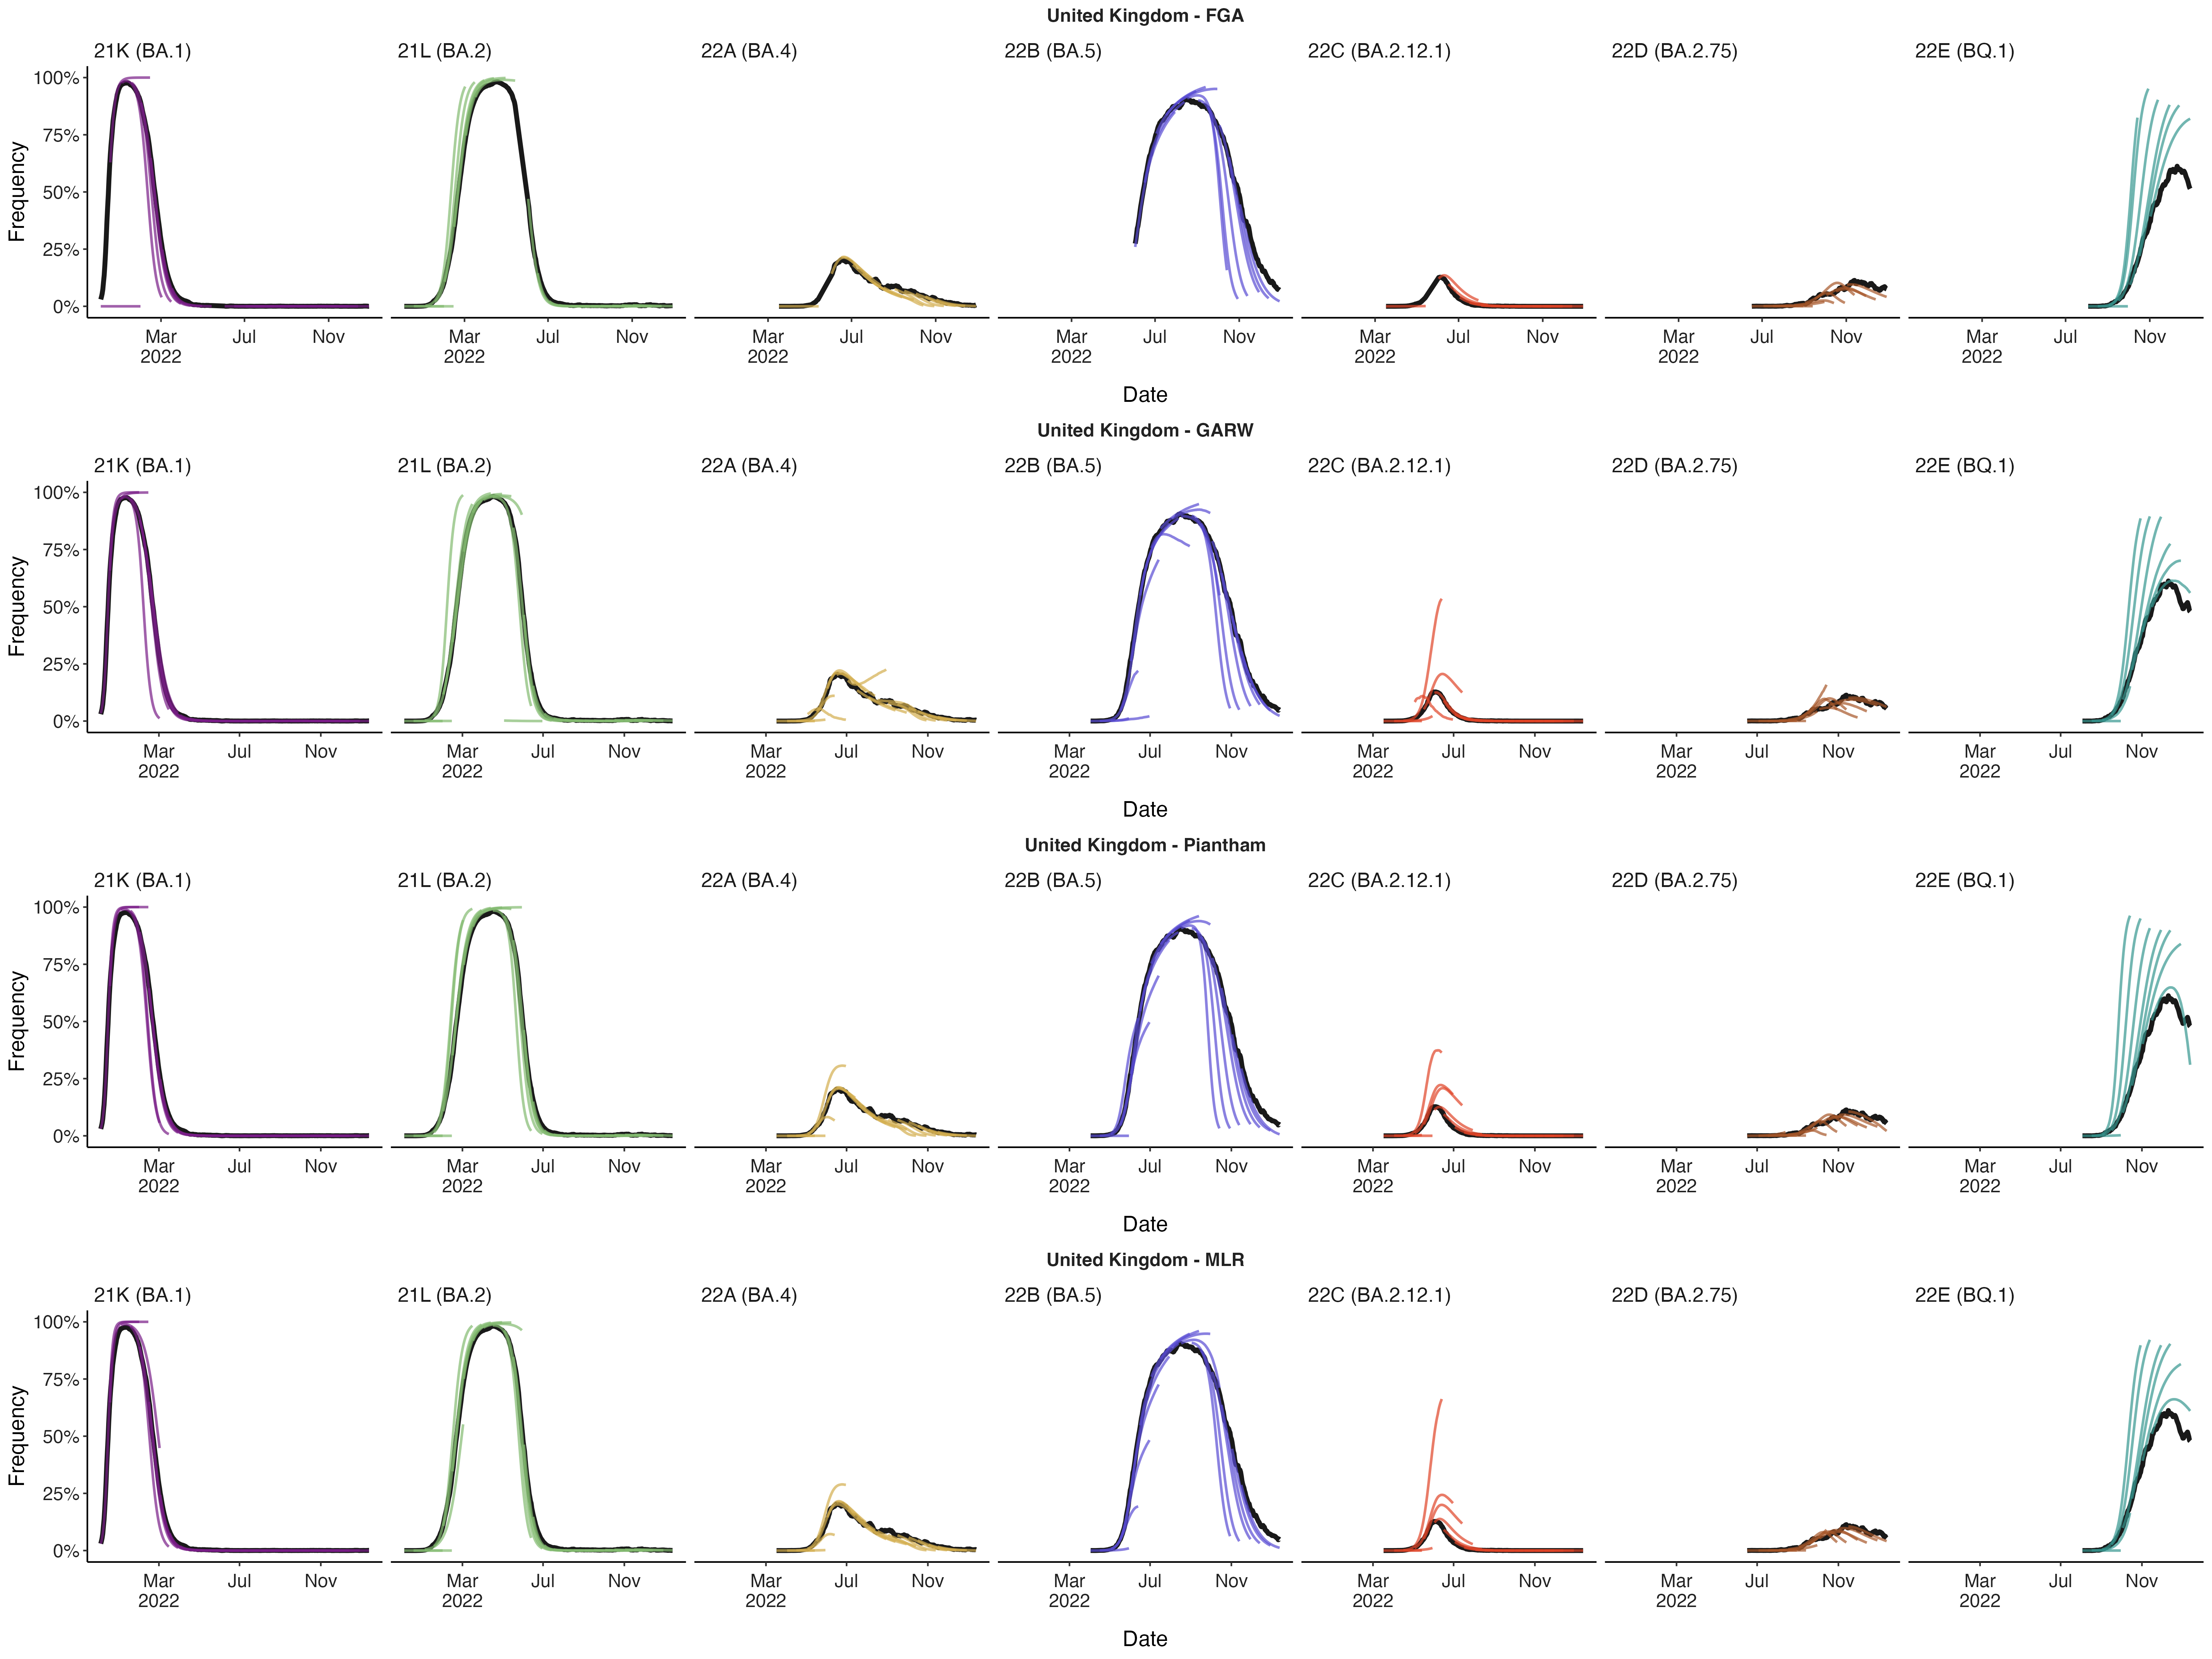
\includegraphics[width=0.9\textwidth=0.01]{supp_figures/supplementary_fig_United Kingdom.png}
	\caption[\textbf{Reconstructing predictions for the United Kingdom}]{
		\textbf{Reconstructing predictions for the United Kingdom}
		(A) +30 day frequency forecasts for variants in bimonthly intervals using the MLR model for the United Kingdom.
		Each forecast trajectory is shown as a different colored line.
		Retrospective smoothed frequency is shown as a thick black line.
	}
	\label{fig:S6}
\end{figure}


% \paragraph*{S7 Fig}
% \label{fig:S7}
% {\bf Reconstructing predictions for Vietnam}
% (A) +30 day frequency forecasts for variants in bimonthly intervals using the MLR model for Vietnam.
% Each forecast trajectory is shown as a different colored line.
% Retrospective smoothed frequency is shown as a thick black line.

\begin{figure}[th!]
	\centering
	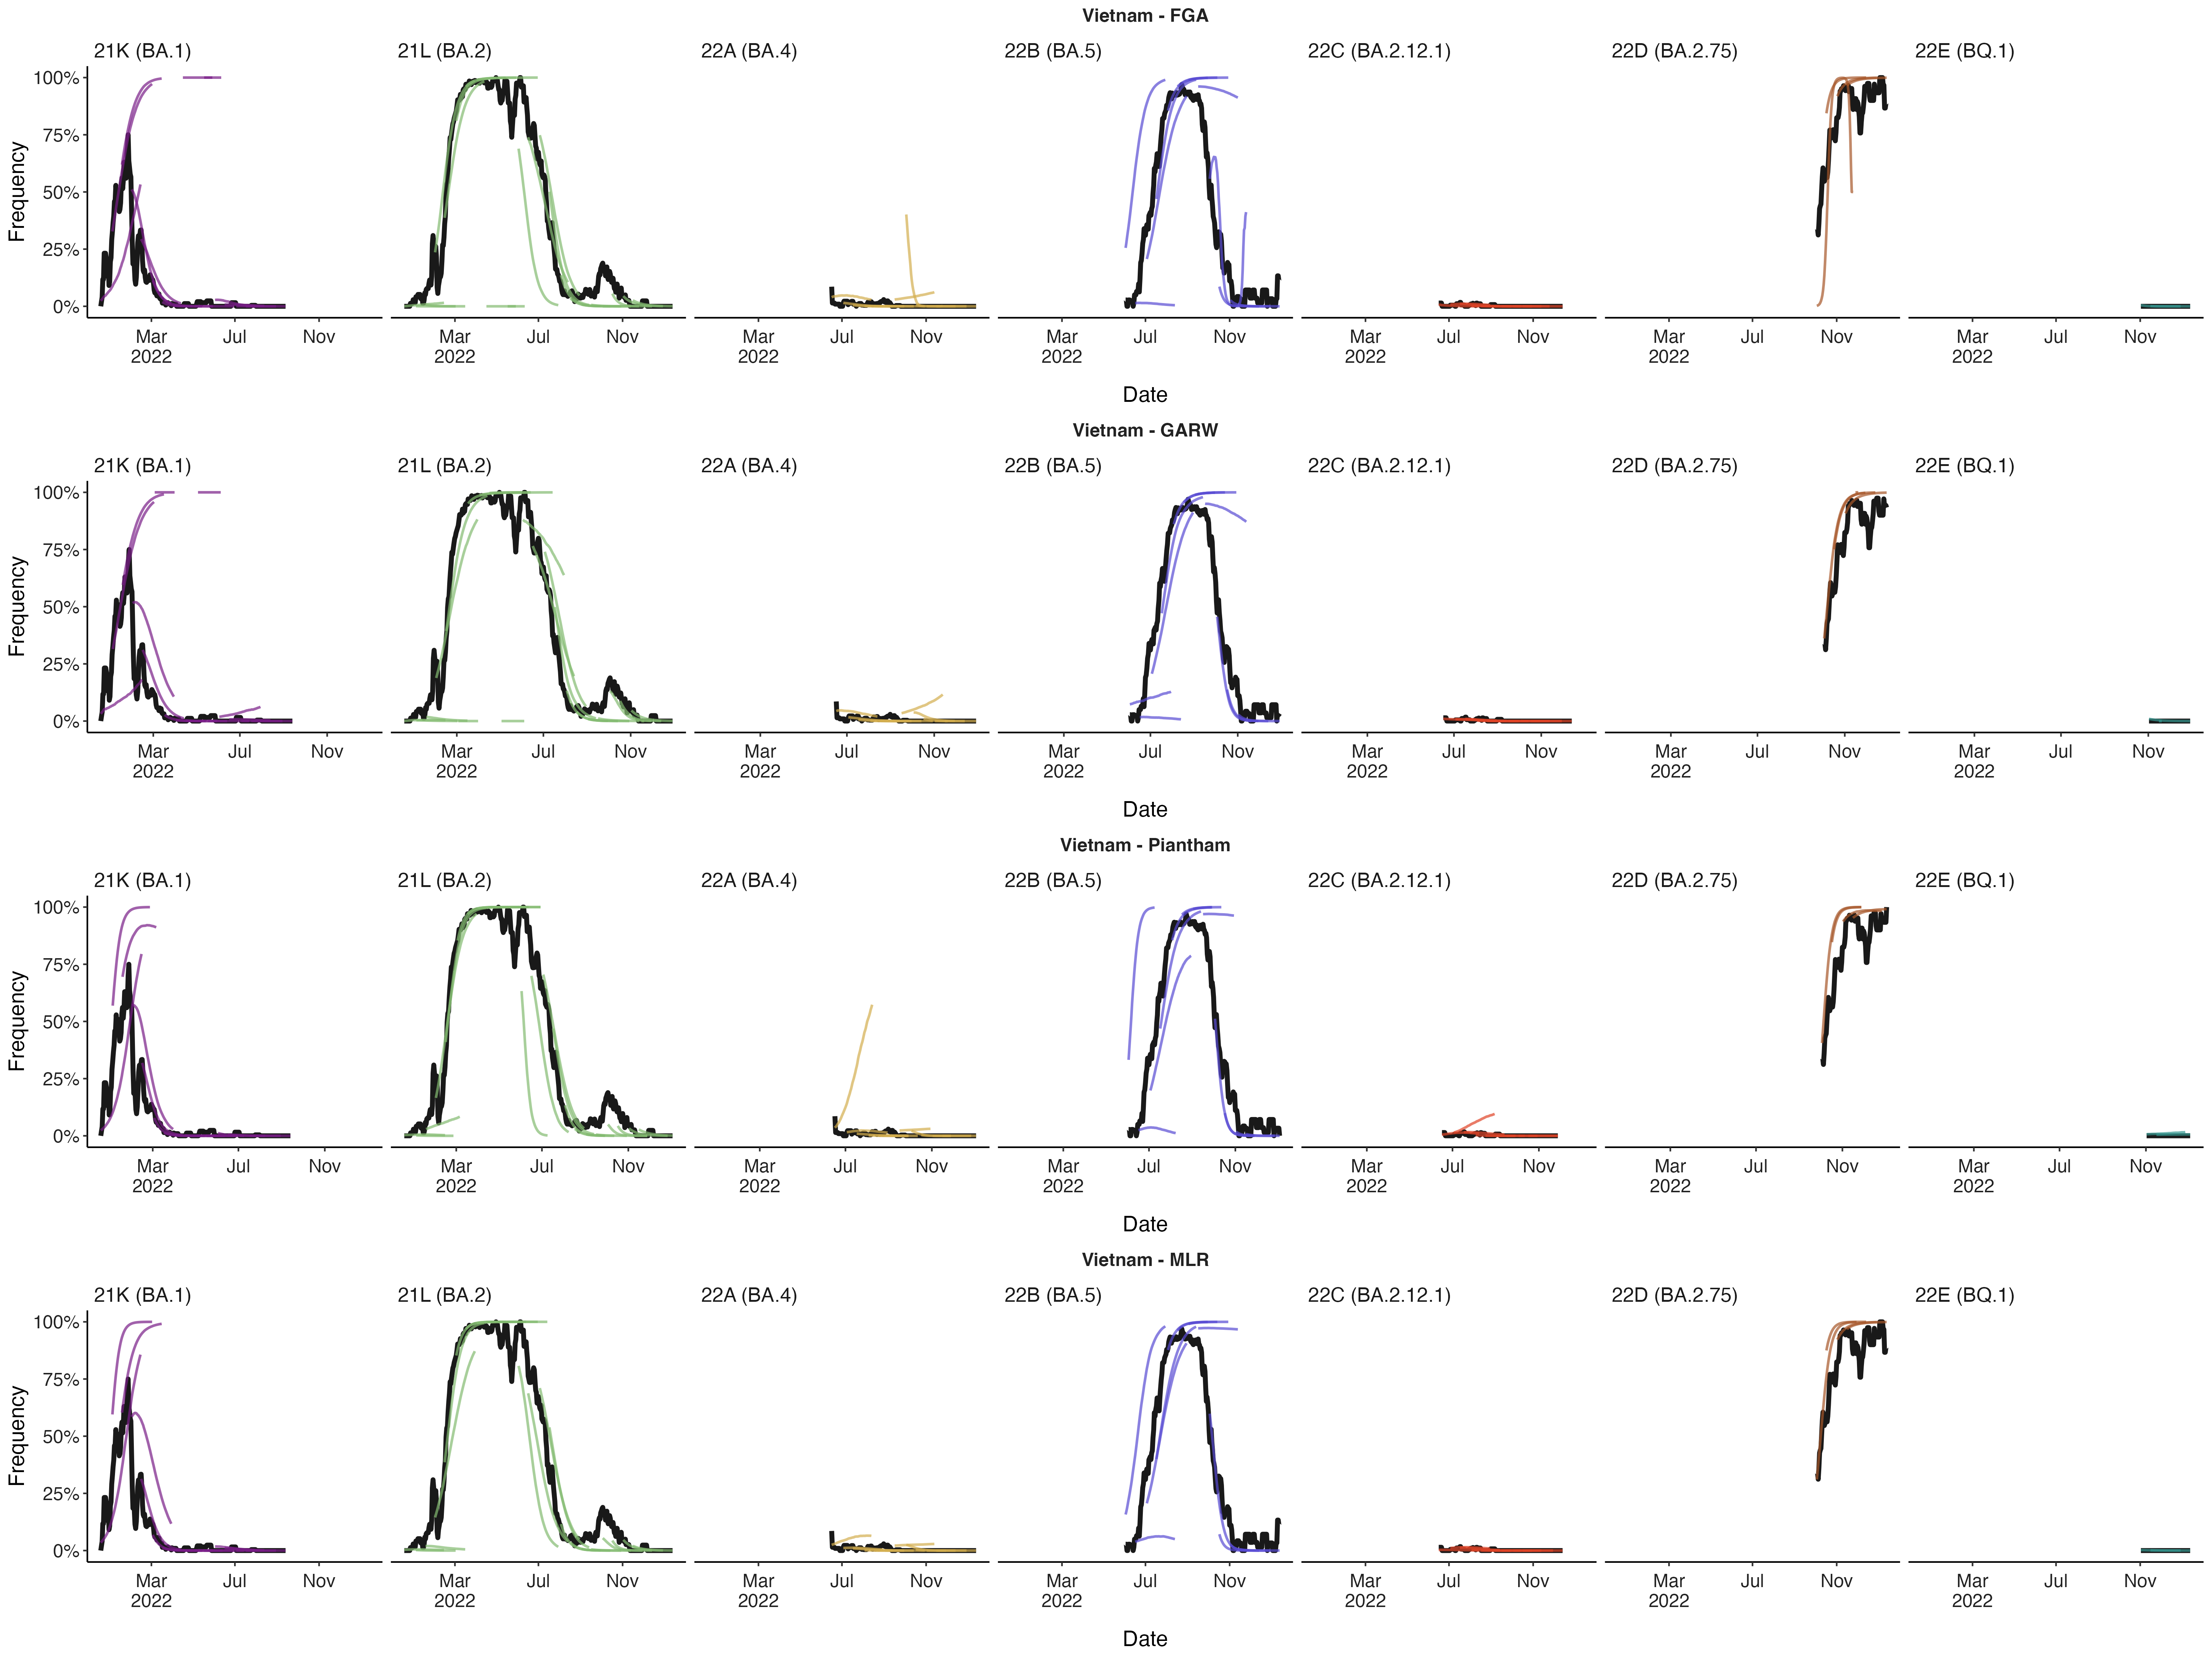
\includegraphics[width=0.9\textwidth=0.01]{supp_figures/supplementary_fig_Vietnam.png}
	\caption[\textbf{Reconstructing predictions for Vietnam}]{
		\textbf{Reconstructing predictions for Vietnam}
		(A) +30 day frequency forecasts for variants in bimonthly intervals using the MLR model for Vietnam.
		Each forecast trajectory is shown as a different colored line.
		Retrospective smoothed frequency is shown as a thick black line.
	}
	\label{fig:S7}
\end{figure}

% \paragraph*{S8 Fig}
% \label{fig:S8}
% {\bf Posterior and predictive coverage for estimates across countries and models}
% (A) The proportion of estimates lying within the 95\% confidence intervals (CIs) of posterior latent frequencies across lag times (-30,-30).
% (B) The proportion of estimates lying within the 95\% confidence intervals (CIs) of posterior predictive sample frequencies across lag times (-30,-30).
% We generate the posterior predictive sample frequencies by sampling random counts for each variant using their posterior latent frequencies conditioning on the total sequences being those observed retrospectively.

\begin{figure}[th!]
	\centering
	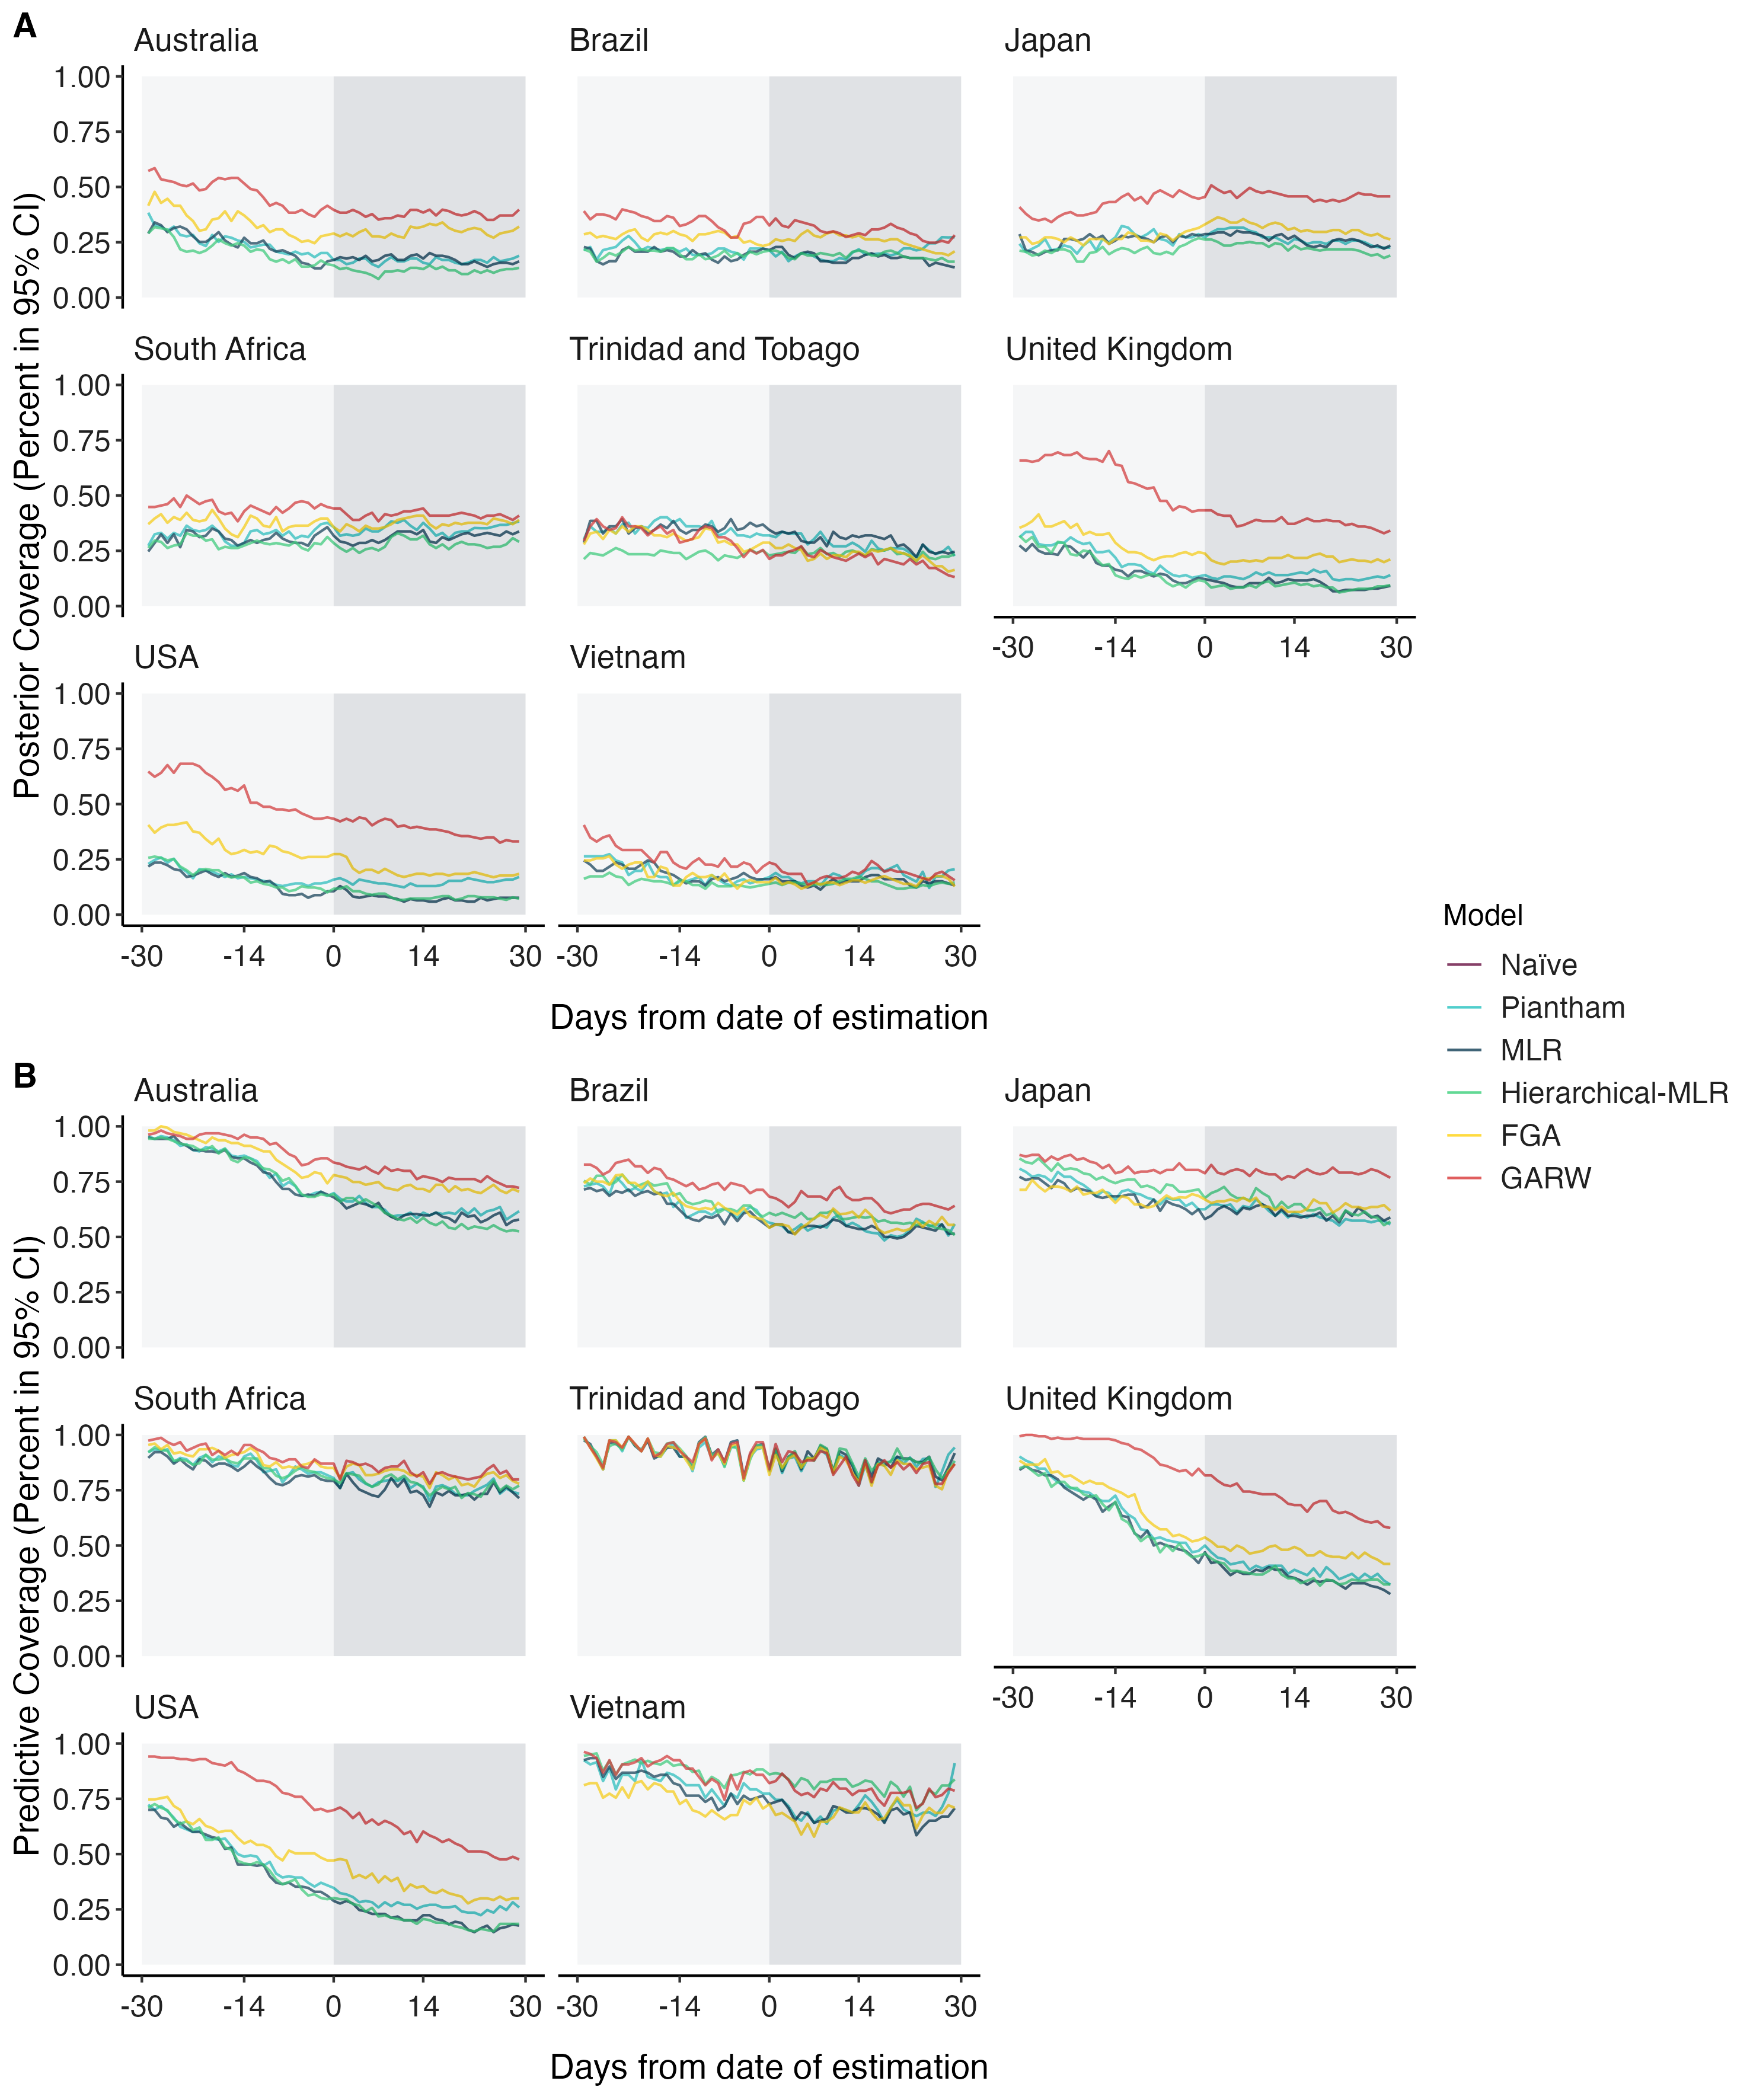
\includegraphics[width=0.8\textwidth]{supp_figures/coverage_supp_2.png}
	\caption[\textbf{Posterior and predictive coverage for estimates across countries and models}]{
		\textbf{Posterior and predictive coverage for estimates across countries and models}
		(A) The proportion of estimates lying within the 95\% confidence intervals (CIs) of posterior latent frequencies across lag times (-30,-30).
		(B) The proportion of estimates lying within the 95\% confidence intervals (CIs) of posterior predictive sample frequencies across lag times (-30,-30).
		We generate the posterior predictive sample frequencies by sampling random counts for each variant using their posterior latent frequencies conditioning on the total sequences being those observed retrospectively.
	}
	\label{fig:S8}
\end{figure}

% \paragraph*{S9 Fig}
% \label{fig:S9}
% {\bf Comparing the accuracy of short-term forecast models under retrospective vs real-time clade assignments.}
% (A-H) Mean absolute error for MLR as a function of days
% since date of estimation, starting from 30 day hindcasts to 30 days forecasts. Intervals shown have
% width of two standard errors of the mean. We compare retrospective Nextstrain clade assignments
% made today (‘Current Nextclade’) to Nextstrain clade assignments available in Oct 2022 (‘Real-
% time Nextclade‘). We find that errors are qualitatively similar regardless of Nextclade version with
% errors being potentially higher for the current Nextclade version.

\begin{figure}[t!]
	\centering
	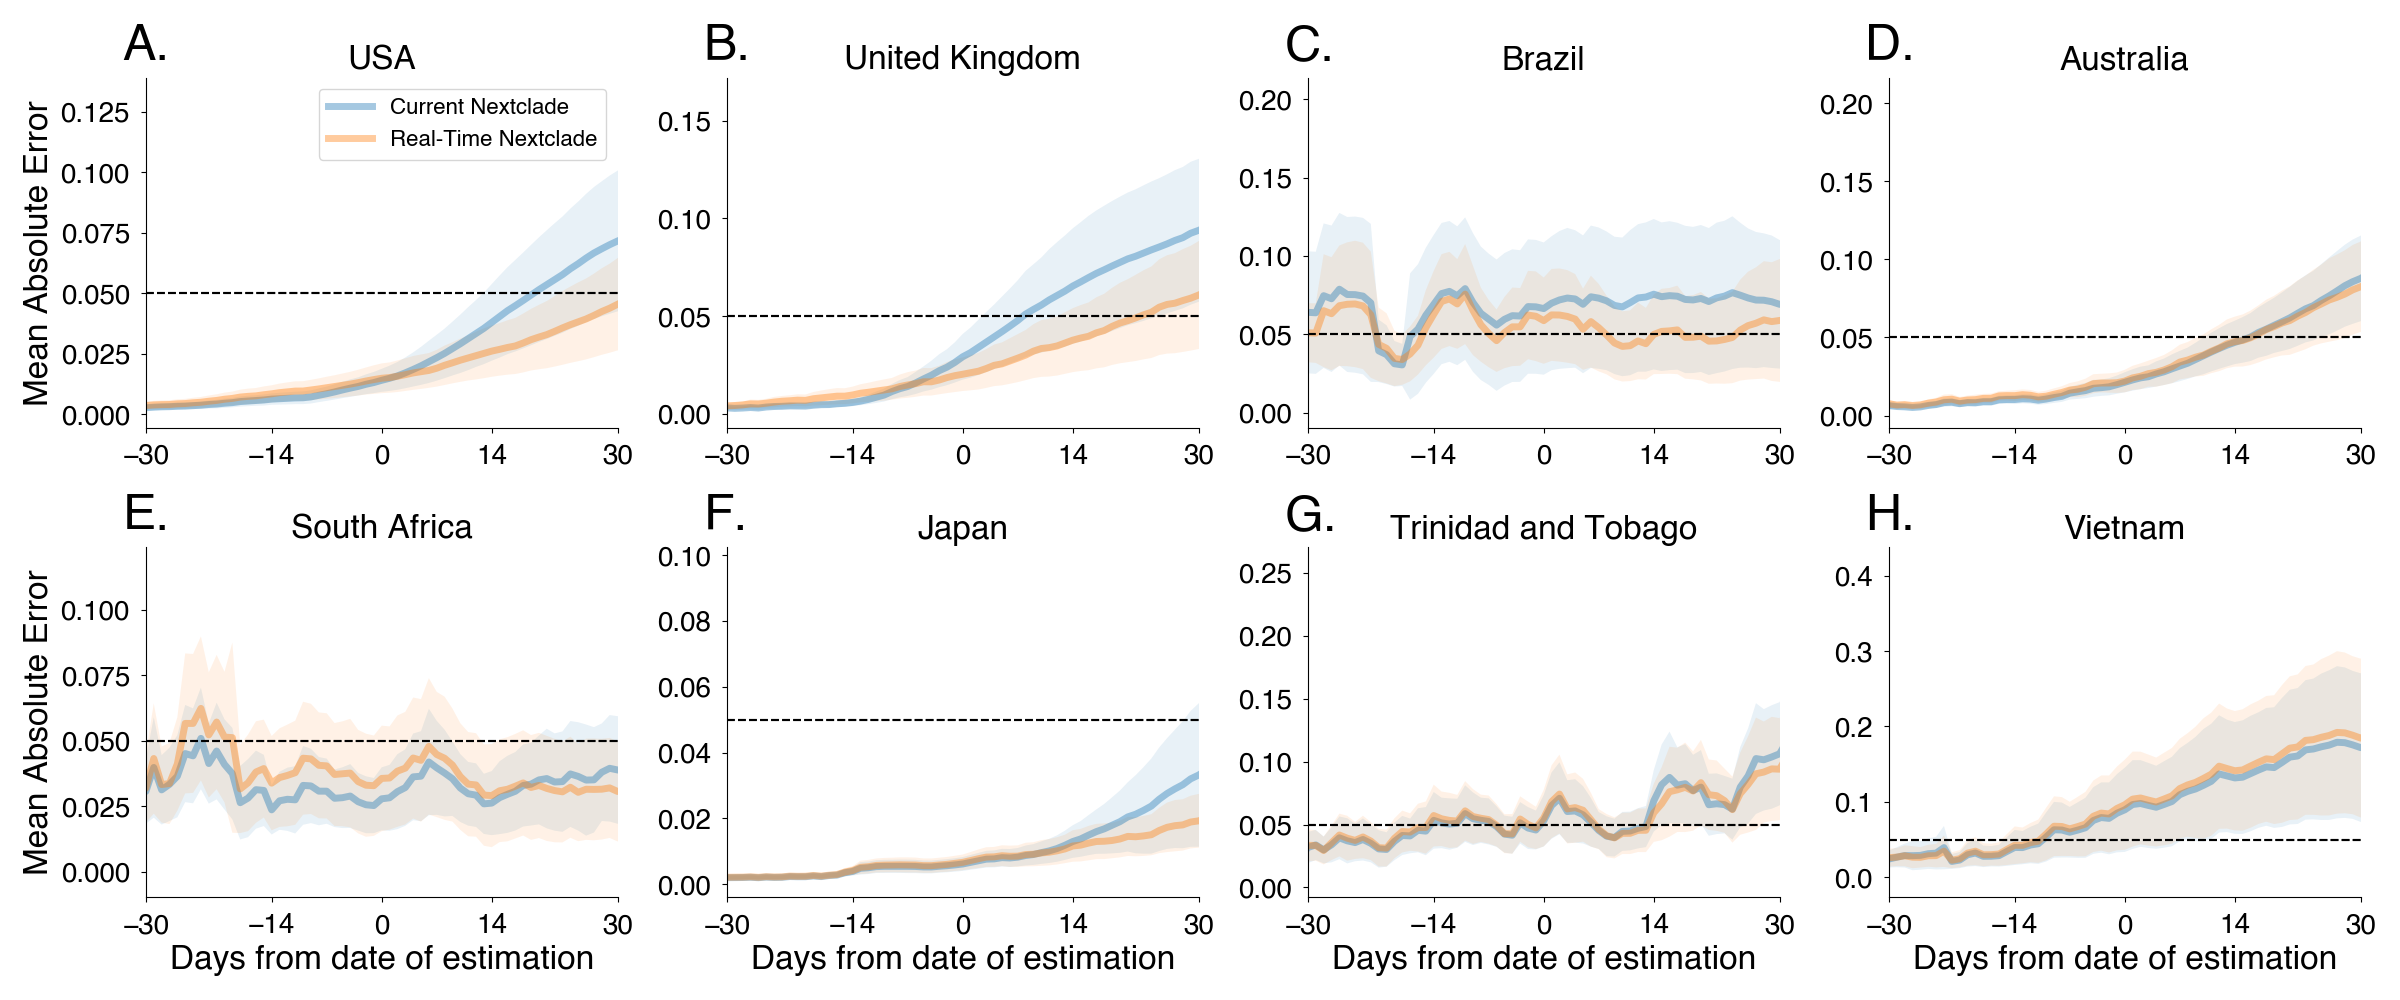
\includegraphics[width=0.9\textwidth=0.01]{./supp_figures/mean_absolute_error_at_lead_nextclade_version_comparison.png}
	\caption[\textbf{Comparing the accuracy of short-term forecast models under retrospective vs real-time clade assignments.}]{
		\textbf{Comparing the accuracy of short-term forecast models under retrospective vs real-time clade assignments.}
        (A-H) Mean absolute error for MLR as a function of days since date of estimation, starting from 30 day hindcasts to 30 days forecasts.
        Intervals shown have width of two standard errors of the mean.
			  We compare retrospective Nextstrain clade assignments made today (`Current Nextclade') to Nextstrain clade assignments available in Oct 2022 (`Real-time Nextclade').
        We find that errors are qualitatively similar regardless of Nextclade version with errors being potentially higher for the current Nextclade version.
	}
	\label{fig:S9}
\end{figure}

\def\forecastcomparisonnextclade#1#2#3{
    \begin{figure}[t!]
        \centering
        \includegraphics[width=0.9\textwidth=0.01]{./supp_figures/forecast-comparison-by-nextclade-version-#3.png}
	\caption[\textbf{Forecasts for #2 using clade designations under retrospective vs real-time clade assignments}]{
            \textbf{Forecasts for #2 using clade designations under retrospective vs real-time clade assignments}
        Forecasts from MLR fit to data generated using retrospective Nextstrain clade designations (`Current Nextclade') (A) and Nextstrain clade assignments available in Oct 2022 (`Real-time Nextclade') (B).
        }
        \label{fig:#1}
    \end{figure}
}

\forecastcomparisonnextclade{S10}{Australia}{Australia}
\forecastcomparisonnextclade{S11}{Brazil}{Brazil}
\forecastcomparisonnextclade{S12}{Japan}{Japan}
\forecastcomparisonnextclade{S13}{South Africa}{South_Africa}
\forecastcomparisonnextclade{S14}{Trinidad and Tobago}{Trinidad_and_Tobago}
\forecastcomparisonnextclade{S15}{United States}{USA}
\forecastcomparisonnextclade{S16}{United Kingdom}{United_Kingdom}
\forecastcomparisonnextclade{S17}{Vietnam}{Vietnam}

% \paragraph*{S10 Fig}
% \label{fig:S10}
% {\bf Forecasts for Australia using clade designations under retrospective vs real-time clade assignments}
% Forecasts from MLR fit to data generated using retrospective Nextstrain clade designations (‘Current Nextclade’) (A) and Nextstrain clade assignments available
% in Oct 2022 (‘Real-time Nextclade‘) (B).
%
% \paragraph*{S11 Fig}
% \label{fig:S11}
% {\bf Forecasts for Brazil using clade designations under retrospective vs real-time clade assignments}
% Forecasts from MLR fit to data generated using retrospective Nextstrain
% clade designations (‘Current Nextclade’) (A) and Nextstrain clade assignments available in Oct
% 2022 (‘Real-time Nextclade‘) (B).
%
% \paragraph*{S12 Fig}
% \label{fig:S12}
% {\bf Forecasts for Japan using clade designations under retrospective vs real-time clade assignments}
% Forecasts from MLR fit to data generated using retrospective Nextstrain
% clade designations (‘Current Nextclade’) (A) and Nextstrain clade assignments available in Oct
% 2022 (‘Real-time Nextclade‘) (B).
%
% \paragraph*{S13 Fig}
% \label{fig:S13}
% {\bf Forecasts for South Africa using clade designations under retrospective vs real-time clade assignments }
% Forecasts from MLR fit to data generated using retrospective Nextstrain clade designations (‘Current Nextclade’) (A) and Nextstrain clade assignments available
% in Oct 2022 (‘Real-time Nextclade‘) (B).
%
% \paragraph*{S14 Fig}
% \label{fig:S14}
% {\bf Forecasts for Trinidad and Tobago using clade designations under retrospective vs real-time clade assignments}
% Forecasts from MLR fit to data generated using retrospective Nextstrain clade designations (‘Current Nextclade’) (A) and Nextstrain clade assign-
% ments available in Oct 2022 (‘Real-time Nextclade‘) (B).
%
% \paragraph*{S15 Fig}
% \label{fig:S15}
% {\bf Forecasts for the United States using clade designations under retrospective vs real-time clade assignments}
% Forecasts from MLR fit to data generated using retrospective Nextstrain clade designations (‘Current Nextclade’) (A) and Nextstrain clade assignments available
% in Oct 2022 (‘Real-time Nextclade‘) (B).
%
% \paragraph*{S16 Fig}
% \label{fig:S16}
% {\bf Forecasts for the United Kingdom using clade designations under retrospective vs real-time clade assignments }
% Forecasts from MLR fit to data generated using retrospective Nextstrain clade designations (‘Current Nextclade’) (A) and Nextstrain clade assignments
% available in Oct 2022 (‘Real-time Nextclade‘) (B).
%
% \paragraph*{S17 Fig}
% \label{fig:S17}
% {\bf Forecasts for Vietnam using clade designations under retrospective vs real-time clade assignments}
% Forecasts from MLR fit to data generated using retrospective Nextstrain clade designations (‘Current Nextclade’) (A) and Nextstrain clade assignments available
% in Oct 2022 (‘Real-time Nextclade‘) (B).


